\chapter{Conceptos Previos}\label{cap3}
\minitoc

En este apartado del trabajo se van a asentar las bases teóricas y conceptos necesarios para poder, partiendo de esta base definir las necesidades de nuestra carga de pago, así como buscar la solución optima para satisfacer la solución de diseño.


\newpage


\section{Calidad de Imagen}
\subsection{\textit{Aliasing}}


\begin{figure}[H]
    \centering
    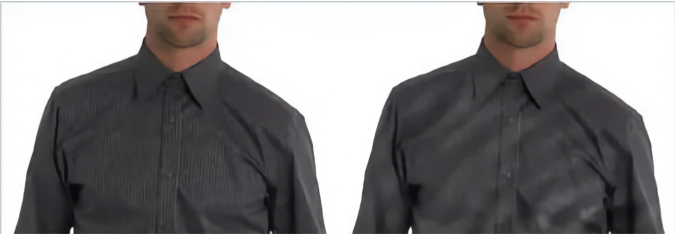
\includegraphics[width=0.7\textwidth]{3.Conceptos_Previos/Moire effect.jpg}
    \caption{Ejemplo del efecto del aliasing sobre un patrón visual.\\ Fuente: \cite{kitdeactores2025moire}}
    \label{fig:Aliasing}
\end{figure}

El \textit{aliasing} es un fenómeno que ocurre cuando una señal con componentes de alta frecuencia es muestreada a una tasa insuficiente, lo que provoca que las frecuencias originales se mezclen y aparezcan como frecuencias más bajas en el espectro reconstruido. En términos de imágenes satelitales, el \textit{aliasing} puede causar artefactos visuales o distorsiones en los datos, degradando la calidad de la imagen capturada. Este problema está directamente relacionado con la frecuencia de Nyquist, que establece que la tasa de muestreo debe ser al menos el doble de la frecuencia espacial máxima presente en la escena para evitar \textit{aliasing}.

\subsection{\textit{Ground Sampling Distance} (GSD)}

\begin{figure}[H]
    \centering
    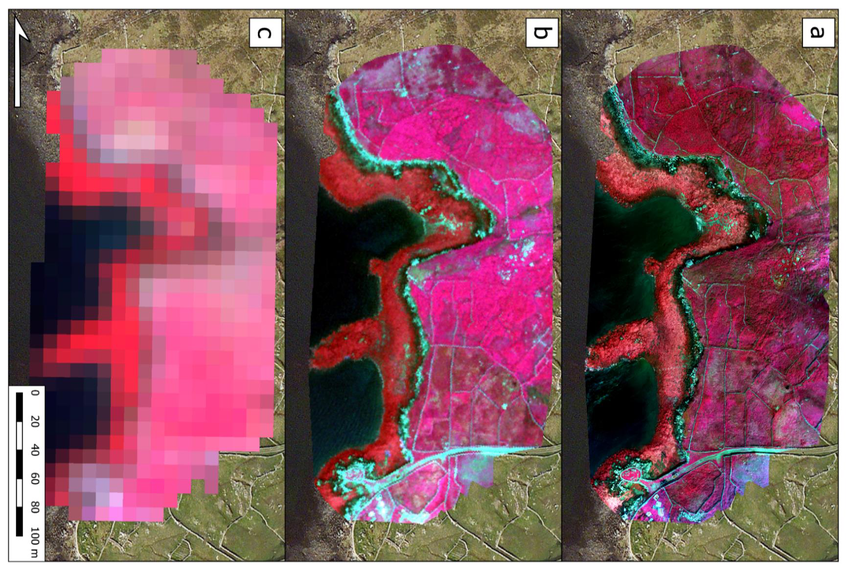
\includegraphics[width=0.7\textwidth]{3.Conceptos_Previos/Comparison-of-the-multispectral-ground-sampling-distance-GSD-from-each-of-the-three.ppm.png}
    \caption{Efectos de distintos GSD en imágenes tomadas por satélite.\\ Fuente: \cite{rossiter2020gsd_comparison}}
    \label{fig:gsdexample}
\end{figure}

La \textbf{Ground Sampling Distance (GSD)} es la distancia en terreno que corresponde a un solo píxel en la imagen capturada por el satélite, determinando la resolución espacial del sistema. Se calcula mediante la relación geométrica entre el tamaño del píxel del detector (\( p \)), la altura orbital (\( h \)) y la distancia focal del telescopio (\( f \)):
\begin{align}
\text{GSD} = \frac{p \cdot h}{f}
\end{align}


\subsection{Frecuencia de Nyquist($f_{Ny}$)}

La \textbf{frecuencia de Nyquist} es un concepto fundamental en la teoría de muestreo que define la máxima frecuencia espacial que un sistema de imagen puede capturar sin distorsión por \textit{aliasing}. En el contexto de un satélite de observación terrestre, esta frecuencia está directamente ligada a la resolución espacial (GSD) y determina la capacidad del sistema para preservar detalles finos en la escena observada.

La frecuencia de Nyquist (\( f_{\text{Nyquist}} \)) se calcula como:
s
\begin{align}
f_{\text{Nyquist}} = \frac{1}{2 \cdot p}
\end{align}

donde el \text{tamaño del pixel} actúa como el intervalo de muestreo espacial.

\subsection{\textit{Modulation Transfer Function} (MTF)}\label{sec:mtfteoria}

La Función de Transferencia de Modulación (MTF) es una herramienta matemática fundamental para evaluar la calidad óptica de un sistema de observación terrestre. La MTF mide la capacidad del sistema óptico para reproducir el contraste de la imagen en función de la frecuencia espacial \cite{design_workshop_optical_2023} \cite{zorita_mtf_2023}.

\begin{figure}[H]
    \centering
    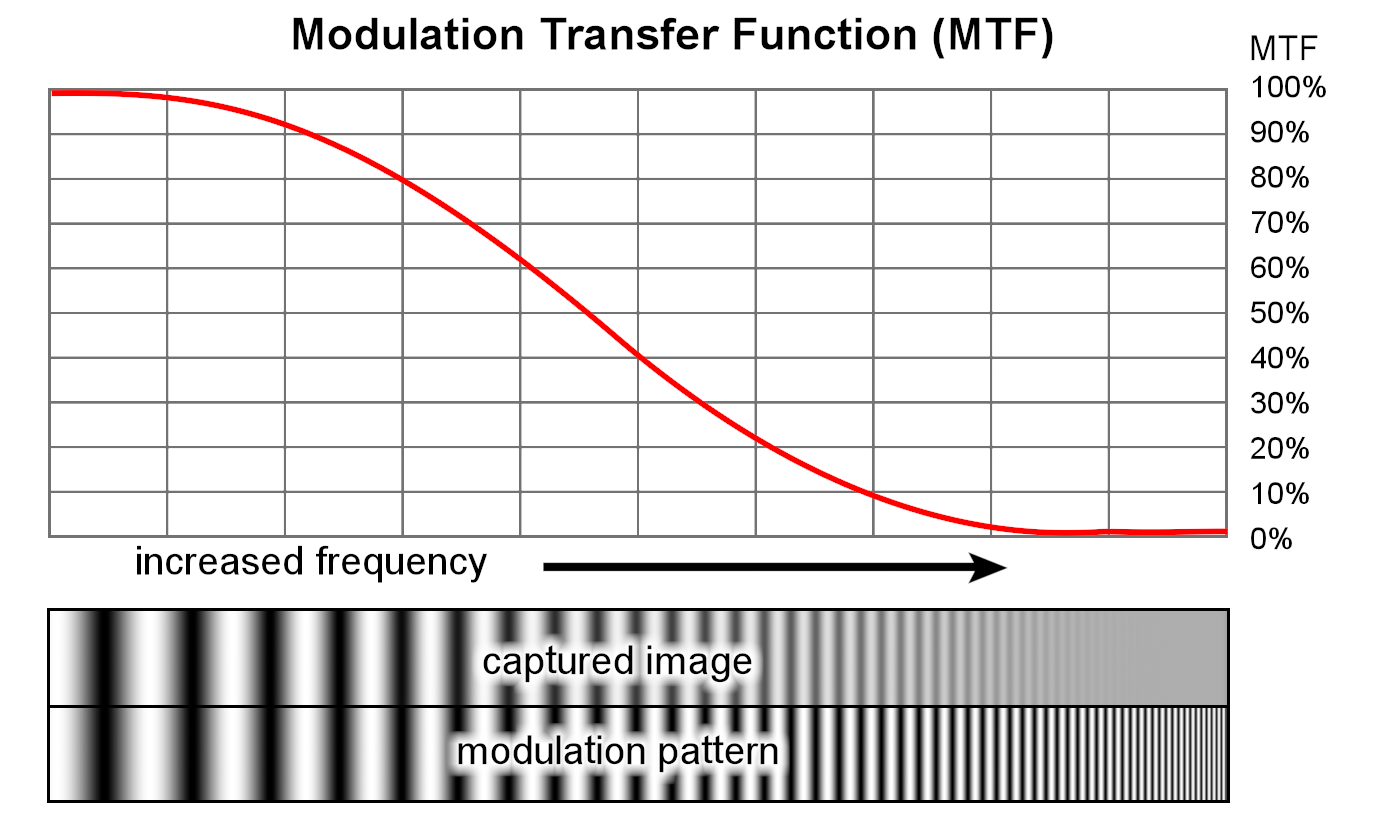
\includegraphics[width=0.7\textwidth]{3.Conceptos_Previos/MTF.png}
    \caption{Representación visual de la MTF.\\ Fuente: \cite{EdmundOptics2023}.}
    \label{fig:MTF}
\end{figure}

En términos simples, la MTF determina cómo un sistema óptico transfiere el contraste desde el objeto hasta la imagen final. Cuando se observa un patrón de franjas blancas y negras (alto contraste), la MTF indica qué porcentaje de ese contraste se preserva en la imagen final. A medida que aumenta la frecuencia espacial (franjas más densas), el contraste tiende a disminuir.


La MTF total del sistema es el producto de las MTF de cada uno de los subsistemas ópticos y electrónicos relevantes. Los principales contribuyentes son:

\begin{itemize}
  \item \textbf{MTF de Difracción:} Limitación física impuesta por el diámetro de la apertura del telescopio y la longitud de onda de observación. Para una apertura circular sin obstrucción, la MTF de difracción se calcula mediante:

  \begin{equation}
  MTF_{\text{difracción}}(f_x) = \frac{2}{\pi} \left[ \arccos\left(\frac{f_x}{f_{co}}\right) - \frac{f_x}{f_{co}} \sqrt{1 - \left(\frac{f_x}{f_{co}}\right)^2} \right]
  \end{equation}

  donde $f_{co} = D / \lambda$ es la frecuencia de corte, $D$ el diámetro de la apertura y $\lambda$ la longitud de onda.

  Para un telescopio obscurado\footnote{obstrucción central que bloquea parte de la luz (normalmente un espejo) que entra al sistema óptico, siendo $d_{obs}$ la medida de dicha obstrucción}, como es el caso de los telescopios Cassegrain y Korsch, su MTF de difracción vendrá definida, en función del diámetro de obscuración $d_{obs}$. Para el presente trabajo se establecerá $R_{obs} = 0,2$ como valor inicial.\cite{Foadi2023DesigningCT}
\begin{equation}
\mathrm{OTF}_{\mathrm{diff}} = \frac{A + B + C}{1 - R^2}
\end{equation}

\begin{equation}\label{mtfrobs}
R = \frac{d_{\mathrm{obs}}}{D_o}
\end{equation}

\begin{equation}
X = \frac{f_x}{f_{\mathrm{oco}}}, \quad Y = \frac{X}{R}, \quad \alpha = \cos^{-1}\left(\frac{1 + R^2 - 4X^2}{2R}\right)
\end{equation}

\begin{equation}
A =
\begin{cases}
\frac{2}{\pi}\left[\cos^{-1}(X) - X\sqrt{1 - X^2}\right], & \text{si } 0 \leq X \leq 1 \\
0, & \text{en otro caso}
\end{cases}
\end{equation}

\begin{equation}
B =
\begin{cases}
\frac{2R^2}{\pi}\left[\cos^{-1}(Y) - Y\sqrt{1 - Y^2}\right], & \text{si } 0 \leq Y \leq 1 \\
0, & \text{en otro caso}
\end{cases}
\end{equation}

\begin{equation}
C =
\begin{cases}
-2R^2, & \text{si } 0 < X \leq \frac{1 - R}{2} \\
\frac{2R}{\pi} \sin\alpha + \frac{1 + R^2}{\pi} \alpha - \frac{2(1 - R^2)}{\pi} \tan^{-1}\left[\left(\frac{1 + R}{1 - R}\right)\tan\left(\frac{\alpha}{2}\right)\right] - 2R^2, & \text{si } \frac{1 - R}{2} < X < \frac{1 + R}{2} \\
0, & \text{si } X \geq \frac{1 + R}{2}
\end{cases}
\end{equation}

Para calcular el requerimiento de MTF, se impone $f_x=f_{Ny}*f$. 
  \item \textbf{MTF de Aberraciones:} Degradación adicional debida a imperfecciones ópticas (aberraciones esféricas, cromáticas, etc.). Un valor típico para sistemas bien diseñados es $MTF_{\text{aberraciones}} \approx 0{,}95$.

  \item \textbf{MTF de Fabricación:} Defectos en la fabricación de los espejos/lentes, típicamente $MTF_{\text{fabricación}} \approx 0{,}98$.

  \item \textbf{MTF de Alineamiento:} Errores en el alineamiento de los elementos ópticos. El valor depende del tipo de telescopio.

  \item \textbf{MTF por Vibraciones y Termoelasticidad:} Cambios entre el alineamiento en tierra y en órbita (vibraciones del lanzamiento y efectos térmicos), típicamente $\approx 0{,}99$ y $\approx 0{,}95$ respectivamente.

  \item \textbf{MTF del Detector:} Es un parámetro definido por el diseño y tecnología del detector, normalmente proporcionado por el fabricante.
  
\end{itemize}
Por tanto, la MTF del sistema será:

\begin{align}
MTF_{\text{sistema}} =\ & MTF_{\text{difracción}} \times MTF_{\text{aberraciones}} \times MTF_{\text{fabricación}} \times MTF_{\text{alineamiento}} \nonumber \\
& \times MTF_{\text{vibraciones}} \times MTF_{\text{termoelástico}} \times MTF_{\text{detector}}
\end{align}


\subsection{\textit{Signal To Noise Ratio} (SNR)}\label{snr}
\begin{figure}[H]
    \centering
    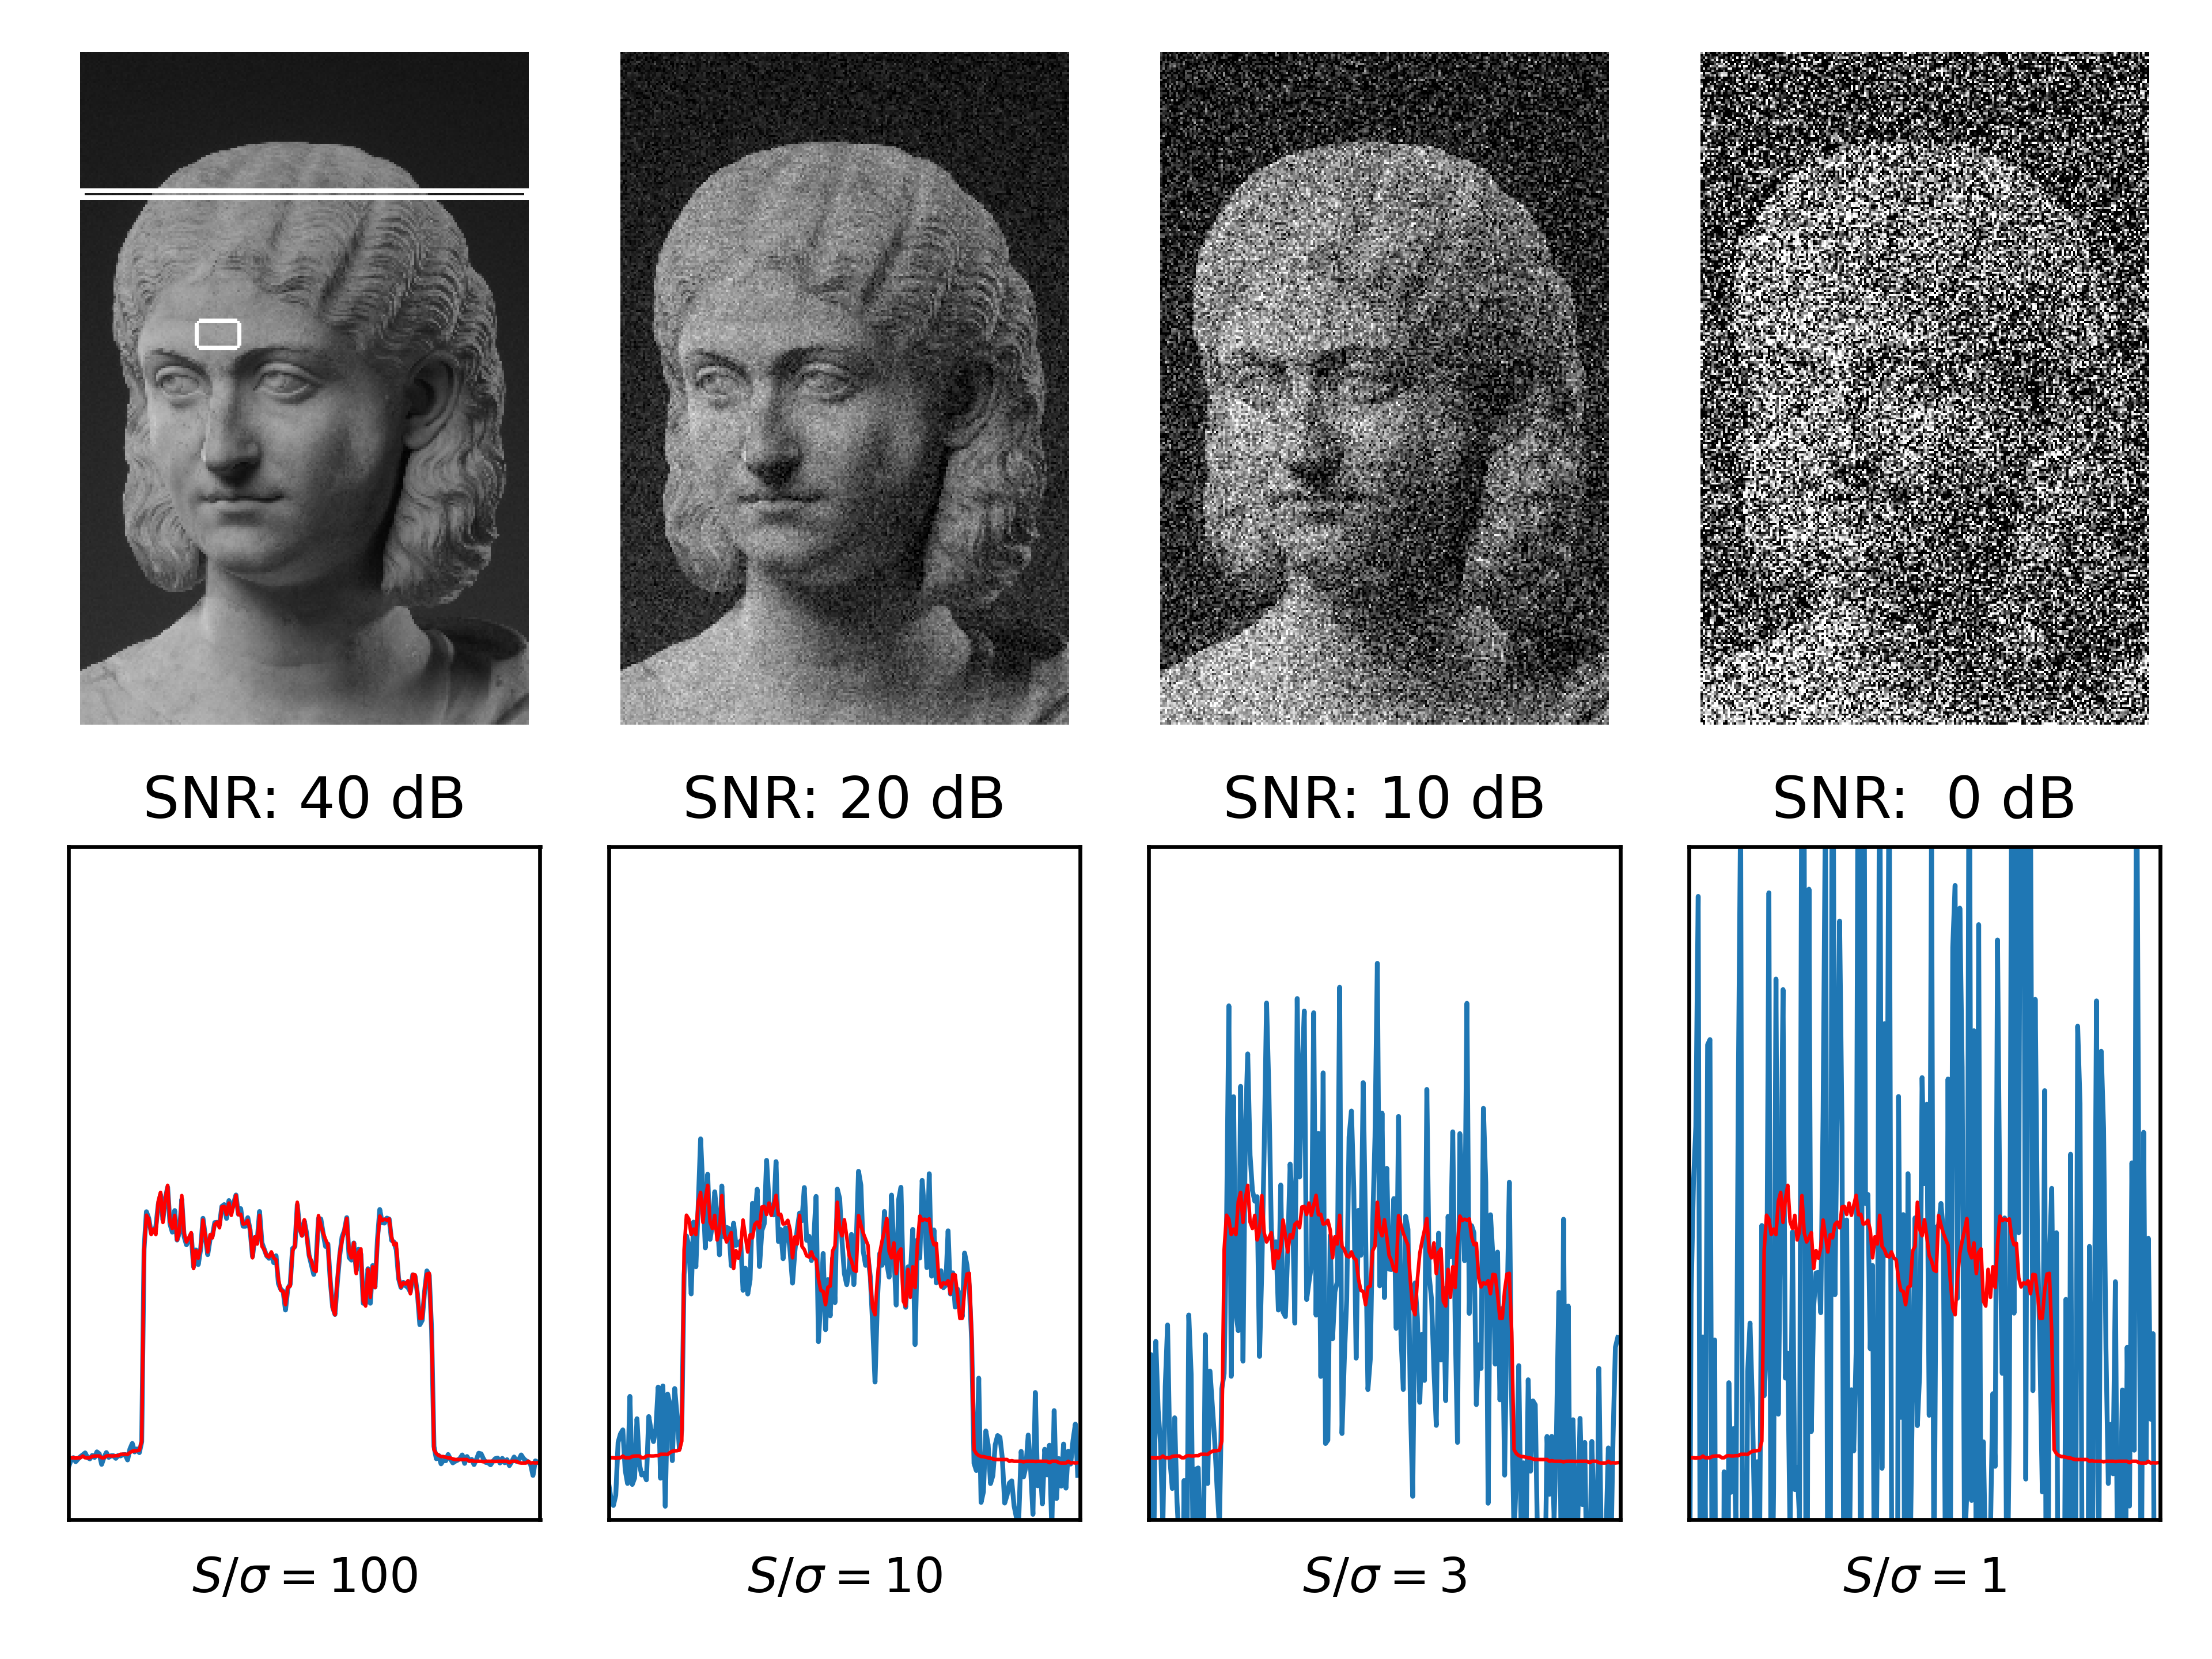
\includegraphics[width=0.5\linewidth]{3.Conceptos_Previos/SNR_image_demonstration.png}
    \caption{Efecto de la SNR.\\ Fuente: \cite{wikipedia2025snr_demonstration}}
    \label{fig:snr}
\end{figure}

La \textit{Signal-to-Noise Ratio} (SNR, o relación señal-ruido) es una métrica clave que indica la calidad radiométrica de un sistema de observación óptica. Representa la relación entre la señal útil (fotones detectados provenientes de la escena) y el ruido total (sumatoria de todas las fuentes de ruido del sistema) en el detector. Un SNR alto significa que la señal es claramente distinguible del ruido, lo que permite obtener imágenes precisas y fiables; un SNR bajo implica que la señal está enmascarada por el ruido, dificultando la detección de detalles y la calidad de los datos obtenidos\cite{design_workshop_optical_2023}\cite{zorita_snr_2023}.

Matemáticamente se expresa como:

\begin{equation}
SNR = \frac{\text{Señal}}{\text{Ruido total}}
\end{equation}

donde la señal y el ruido se expresan en número de electrones generados ($e^-$)en el detector durante el tiempo de integración.

\subsubsection{Cálculo de la Señal}


Se considera una radiancia de referencia \( L_{\mathrm{ref}} \) expresada en \( \si{\watt\per\metre\squared\per\steradian\per\micro\metre} \), centrada en una longitud de onda \( \lambda_c \) con un ancho de banda espectral \( \Delta \lambda \). La radiancia incidente se transmite a través del sistema óptico con una eficiencia total condicionada por la transmisión óptica del telescopio \( \tau \) y la eficiencia cuántica del detector \( \eta \). 

La irradiancia \( I \) en el plano focal se estima mediante:

\begin{equation}
I = \frac{\pi \cdot \tau \cdot \Delta \lambda \cdot L_{\mathrm{ref}}}{1 + 4F\#}
\end{equation}

donde \( F\# = \frac{f}{D} \) es la relación focal del sistema, con \( f \) la distancia focal y \( D \) el diámetro de la apertura.\footnote{Para los sistemas obscurados se utilizará la relación focal equivalente $T\#$, definida mas adelante en la ecuación \ref{relfoc}}.

La cantidad de electrones generados por píxel durante el tiempo de integración se calcula como:

\begin{equation}
N_e = \frac{E \cdot A_p \cdot \eta \cdot \lambda_c \cdot TDI \cdot t_{\mathrm{int}}}{h \cdot c}
\end{equation}

donde:
\begin{itemize}
    \item \( A_p = d_x \cdot d_y \) es el área de un píxel en el detector.
    \item \( TDI \) es el número de etapas del sistema Time Delay Integration.\footnote{Dicho concepto se explicará mas adelante en \ref{sec:tdi}}.
    \item \( t_{\mathrm{int}} = \frac{\mathrm{GSD}}{v_{\mathrm{orb}}} \) es el tiempo de integración basado en la velocidad del satélite sobre el suelo.
    \item \( h \) es la constante de Planck.
    \item \( c \) es la velocidad de la luz.
\end{itemize}

El tiempo de integración \( t_{\mathrm{int}} \) representa la duración durante la cual la imagen de un punto en la superficie terrestre permanece proyectada sobre un mismo píxel del detector mientras el satélite avanza en su órbita. Este tiempo depende directamente de la \textit{Ground Sampling Distance} (GSD) y de la velocidad del satélite sobre el suelo \( v_{\mathrm{orb}} \). Se calcula como:

\begin{equation}
t_{\mathrm{int}} = \frac{\mathrm{GSD}}{v_{\mathrm{orb}}}
\end{equation}

La velocidad orbital del satélite a una altitud \( H\) se estima aplicando la tercera ley de Kepler:

\begin{equation}
v_{\mathrm{orb}} = \sqrt{\frac{\mu}{R_T + H}}
\end{equation}

donde \( \mu = 3.986 \times 10^{14} \, \si{m^3/s^2} \) es el parámetro gravitacional estándar de la Tierra y \( R_T = 6371 \, \si{km} \) es el radio medio terrestre. Este tiempo de integración se utiliza directamente en el cálculo de \( N_e \), y representa el tiempo efectivo durante el cual se acumulan fotones en cada píxel del detector.

\subsubsection{Cálculo del Ruido Total}

El ruido total es la raíz cuadrada de la suma de las varianzas de todas las fuentes de ruido independientes del sistema, expresadas en número de electrones:

\begin{equation}
\text{Ruido total} = \sqrt{\sigma_{\text{fotónico}}^2 + \sigma_{\text{stray}}^2 + \sigma_{\text{dark}}^2 + \sigma_{\text{lectura}}^2 + \sigma_{\text{amp}}^2 + \sigma_{\text{vídeo}}^2 + \sigma_{\text{jitter}}^2 + \sigma_{\text{EMC}}^2 + \sigma_{\text{cuant}}^2}
\end{equation}

Las principales fuentes de ruido son:

\begin{itemize}
    \item \textbf{Ruido fotónico (shot noise):} Raíz cuadrada del número de electrones generados por la señal, debido a la naturaleza estadística de la llegada de fotones (\( \sqrt{N_{e^-}} \)).
    \item \textbf{Ruido de corriente de oscuridad:} Asociado a electrones generados térmicamente en el detector, incluso en ausencia de luz.
    \item \textbf{Ruido de lectura:} Introducido por la electrónica de lectura del detector.
    \item \textbf{Otros ruidos electrónicos:} Como preamplificadores, cadena de vídeo, jitter, EMC, etc.
    \item \textbf{Ruido de cuantificación:} Introducido al digitalizar la señal.
\end{itemize}

\subsubsection{Expresión Final de la SNR}

Realizando el cociente entre señal y ruido, resulta la ecuación:

\begin{equation}
SNR = \frac{N_{e^-}}{\sqrt{N_{e^-} + \sigma_{\text{stray}}^2 + \sigma_{\text{dark}}^2 + \sigma_{\text{lectura}}^2 + \sigma_{\text{amp}}^2 + \sigma_{\text{vídeo}}^2 + \sigma_{\text{jitter}}^2 + \sigma_{\text{EMC}}^2 + \sigma_{\text{cuant}}^2}}
\end{equation}


\subsection{\textit{Field of View} (FoV). \textit{Swath}}

\begin{figure}[H]
    \centering
    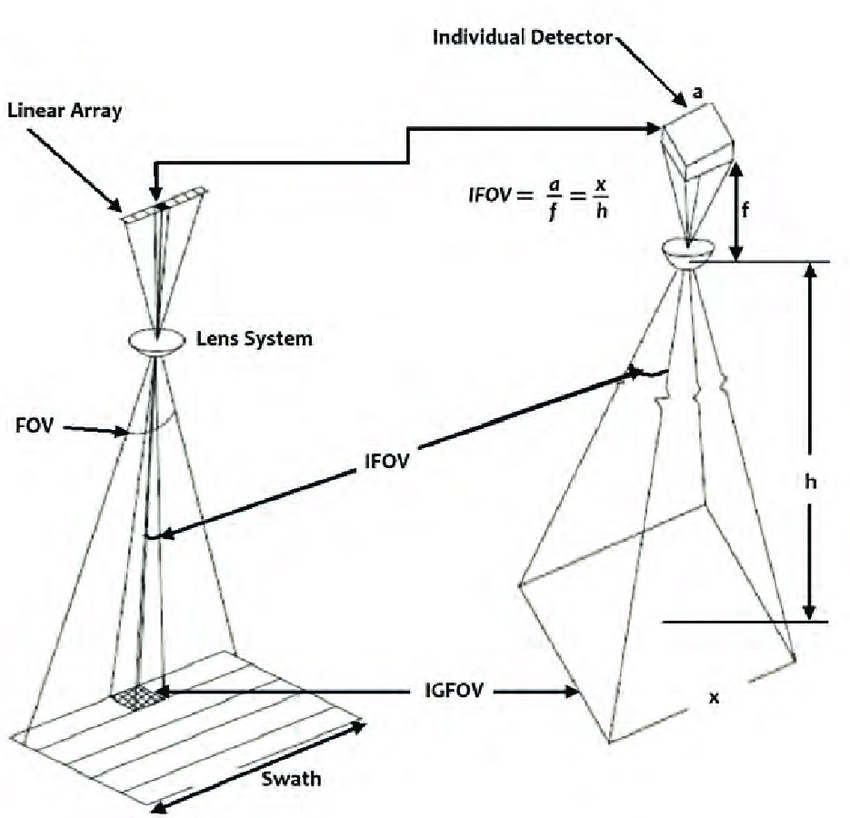
\includegraphics[width=0.7\textwidth]{3.Conceptos_Previos/Swath,fov.png}
    \caption{Esquema visual del \textit{swath} y FoV.\\Fuente: \cite{swath_fov_diagram}.}
    \label{fig:swath}
\end{figure}

El \textit{\textbf{swath}} se define como la anchura de la franja de terreno que el satélite puede observar en una pasada. Se mide en kilómetros y depende tanto de la óptica del instrumento como de la altura orbital. Un \textit{swath} mayor permite cubrir más superficie terrestre en menos tiempo, lo que reduce el tiempo de revisita necesario para obtener mapas completos del área de interés. Se relaciona con el GSD mediante la ecuación:

\begin{equation}
\label{swath}
Swath = GSD \cdot N_{pix} 
\end{equation}

Siendo $N_{pix}$ el numero de píxeles situados en linea perpendicular al sentido de movimiento del satélite.

\textbf{\textit{Field of View} (FoV)} es el ángulo total que abarca el sistema óptico del instrumento, es decir, el ángulo desde el cual la óptica puede captar luz y formar imagen sobre el detector. El FoV se mide en grados o milirradianes y determina, junto con la altura orbital, el swath en tierra.


Ambos valores se relacionan de la siguiente manera:

\begin{equation}
\label{fov}
Swath = 2h \cdot \tan \left( \frac{FoV}{2} \right)
\end{equation}

Siendo $h$ la altura órbital.

En este estudio se asume que solo se observará al \textbf{nadir}, es decir, el instrumento siempre apunta directamente hacia abajo, al punto situado justo debajo del satélite en la superficie terrestre (\textit{sub satellite point}). Esto significa que no se realizarán observaciones oblicuas (\textit{off-nadir}), lo que simplifica el diseño óptico y la planificación de misión. Así mismo, el punto subsatélite es el punto de máxima resolución y mínima distorsión geométrica en la imagen captada, con lo que se maximiza la calidad geométrica y radiométrica de la imagen y se simplifica la calibración y el procesamiento de datos. Además, el cálculo del GSD y del MTF es directo, ya que no hay degradación por ángulo de observación. Así mismo, tampoco se considerará la deformación producida por la esfericidad de la Tierra, considerando la superficie a capturar como plana, ni las deformaciones producidas en los extremos del array debido a su proyección.

\section{Espectro electromagnético. Bandas de absorción}

\begin{figure}[H]
    \centering
    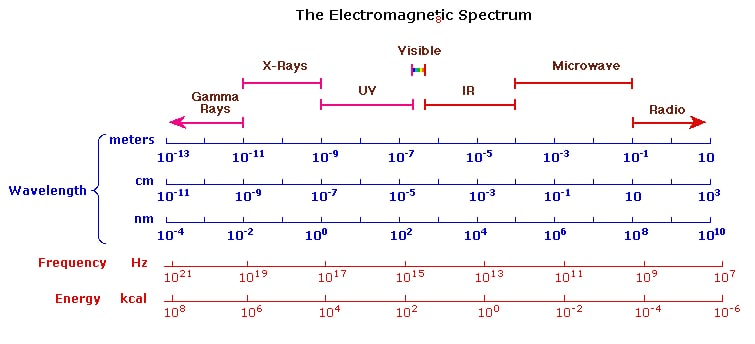
\includegraphics[width=0.7\textwidth]{3.Conceptos_Previos/emspec.jpg}
    \caption{Representación del espectro electromagnético con las longitudes de onda, frecuencias y energías asociadas. \\ Fuente: \cite{WikiLecturesSpectrum}.}
    \label{fig:emspec}
\end{figure}

El espectro electromagnético abarca todas las formas de radiación, desde los rayos gamma (longitudes de onda ultracortas) hasta las ondas de radio (longitudes de onda largas). Cada elemento químico absorbe o emite radiación en frecuencias específicas, actuando como una "huella digital" única. Estas interacciones se miden mediante espectrómetros, que identifican los patrones de absorción para determinar la composición química de un objeto o atmósfera. La detección satelital aprovecha estas propiedades para analizar gases en la Tierra, seleccionando bandas espectrales donde la señal del gas objetivo es clara y diferenciable de interferencias.

\subsubsection{Ventanas de observación y transmitancia atmosférica}
\begin{figure}[H]
    \centering
    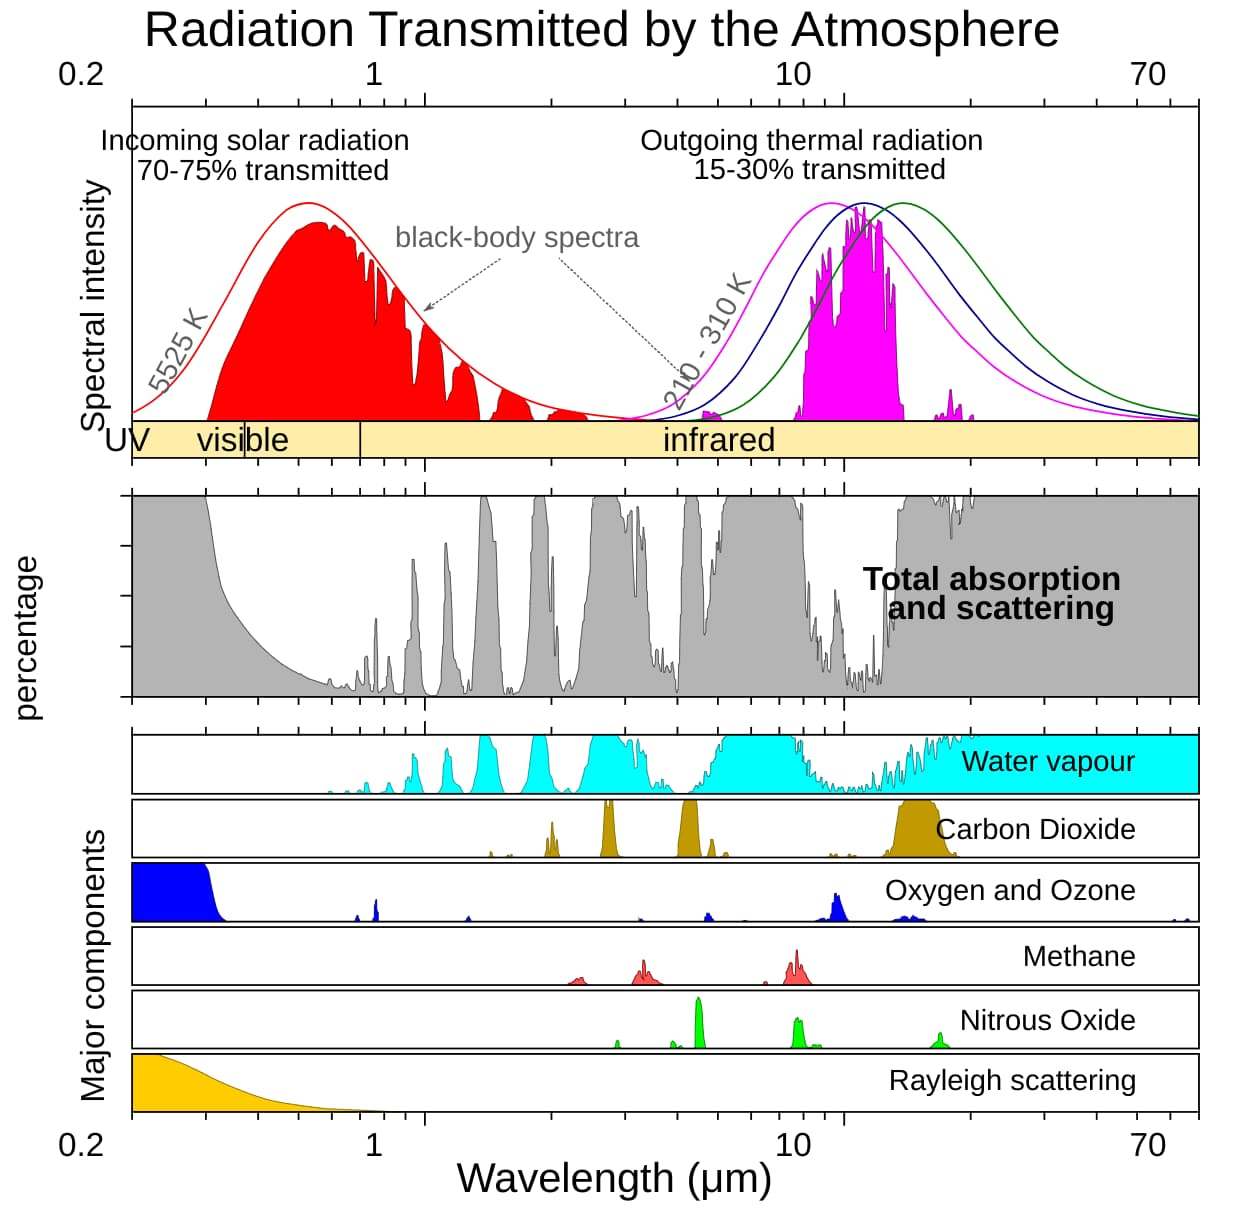
\includegraphics[width=0.7\textwidth]{3.Conceptos_Previos/Atmospheric_Transmission-en.jpg} 
    \caption{Radiación transmitida por la atmósfera y bandas de absorción. \\Fuente: \cite{atmospheric_transmission_spectrum}.}
    \label{fig:atm_transmission}
\end{figure}

La atmósfera terrestre no es transparente a todas las longitudes de onda. Gases como el CO$_2$, el vapor de agua y el ozono absorben fuertemente en regiones específicas, creando "bandas de absorción" que bloquean la radiación. Por ejemplo, el vapor de agua absorbe en el infrarrojo medio (6–8 $\mu$m) y el ozono en el ultravioleta (200–300 nm). Sin embargo, existen "ventanas atmosféricas" donde la radiación atraviesa con menor interferencia, como la región de 8–12 $\mu$m (infrarrojo térmico) y 14–16 $\mu$m (infrarrojo lejano). Estas ventanas son críticas para la teledetección, ya que permiten a los satélites capturar la radiación emitida o reflejada por la superficie terrestre \cite{wilber_surface_1999}.

\subsubsection{Bandas de absorción del CO\textsubscript{2}}

\begin{figure}[H]
    \centering
    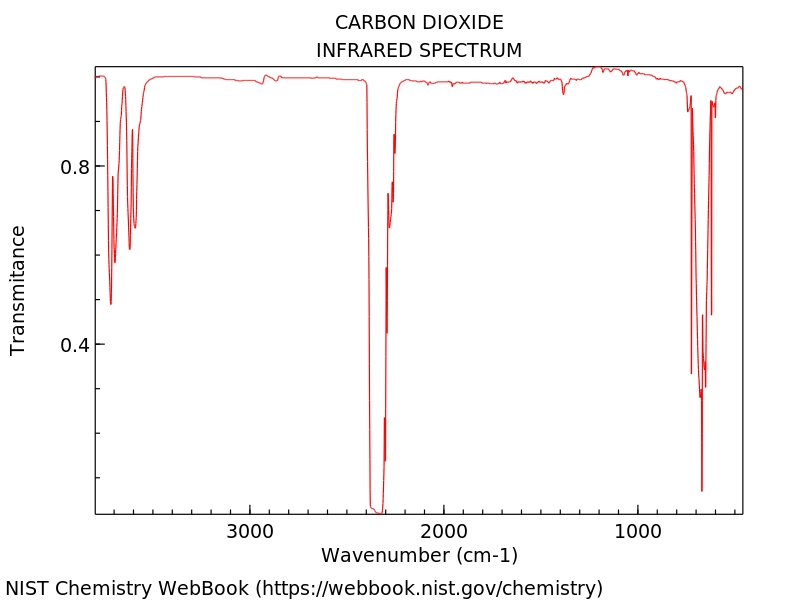
\includegraphics[width=1\textwidth]{3.Conceptos_Previos/cbook.cgi-2.png}
    \caption{Bandas de Transmitancia del CO$_2$ en función del número de onda.\\Fuente: \cite{nist2025co2_spectrum} }
    \label{fig:co2trans}
\end{figure}

El CO$_2$ presenta bandas de absorción características en diferentes regiones espectrales. Las bandas de 1,6 $\mu$m y 2,01 $\mu$m en el infrarrojo cercano son utilizadas por satélites como OCO-2 y GOSAT para medir la concentración columnar de CO$_2$ (XCO$_2$) mediante análisis de reflectancia solar. Estas bandas permiten la detección de CO$_2$ atmosférico aprovechando la absorción en la radiación solar reflejada por la superficie terrestre \cite{oco2_technical_specs_2024}.


La banda de 14--16 $\mu$m, aunque presenta fuerte absorción de CO$_2$, resulta inadecuada para mediciones de concentración desde plataformas espaciales. Esta banda mide principalmente temperatura atmosférica en lugar de concentraciones de CO$_2$, ya que la opacidad atmosférica impide la penetración hasta niveles superficiales donde ocurren las emisiones antropogénicas. Los algoritmos de recuperación requieren perfiles de temperatura extremadamente precisos, introduciendo incertidumbres que complican la separación entre efectos térmicos y variaciones de concentración. La fuerte absorción del CO$_2$ en 15 $\mu$m genera opacidad atmosférica elevada que limita la radiación detectada a niveles de la alta atmósfera, reduciendo significativamente la sensibilidad a las concentraciones cerca de la superficie terrestre \cite{pmc_co2_absorption_2018}.



\section{Detectores}

Los detectores de imágenes utilizados en satélites de observación son dispositivos electrónicos que convierten la radiación electromagnética en señales eléctricas. Este proceso se basa en el efecto fotoeléctrico, mediante el cual los fotones incidentes generan pares electrón-hueco en materiales semiconductores. Los detectores modernos se componen de matrices de píxeles, capaces de acumular carga eléctrica proporcional a la intensidad de la radiación recibida. Su estructura básica incluye una capa fotosensible de silicio u otro material semiconductor, junto con componentes electrónicos para la gestión, amplificación y lectura de estas cargas.

Para operar en el espacio, estos detectores deben superar condiciones particularmente exigentes: radiación cósmica, variaciones extremas de temperatura y ausencia de mantenimiento físico. Además, se requiere alta sensibilidad en las longitudes de onda de interés, bajo nivel de ruido para detectar señales débiles y un consumo energético reducido, dado que las plataformas satelitales disponen de recursos limitados. Parámetros como la resolución espacial, temporal y radiométrica son determinantes en la calidad de los datos adquiridos y su utilidad en distintas aplicaciones científicas y operativas \cite{kuroda_essential_2014}.

\subsection{Tipos de detectores}

\subsubsection{Sensores CCD (Charge-Coupled Device)}

\begin{figure}[H]
    \centering
    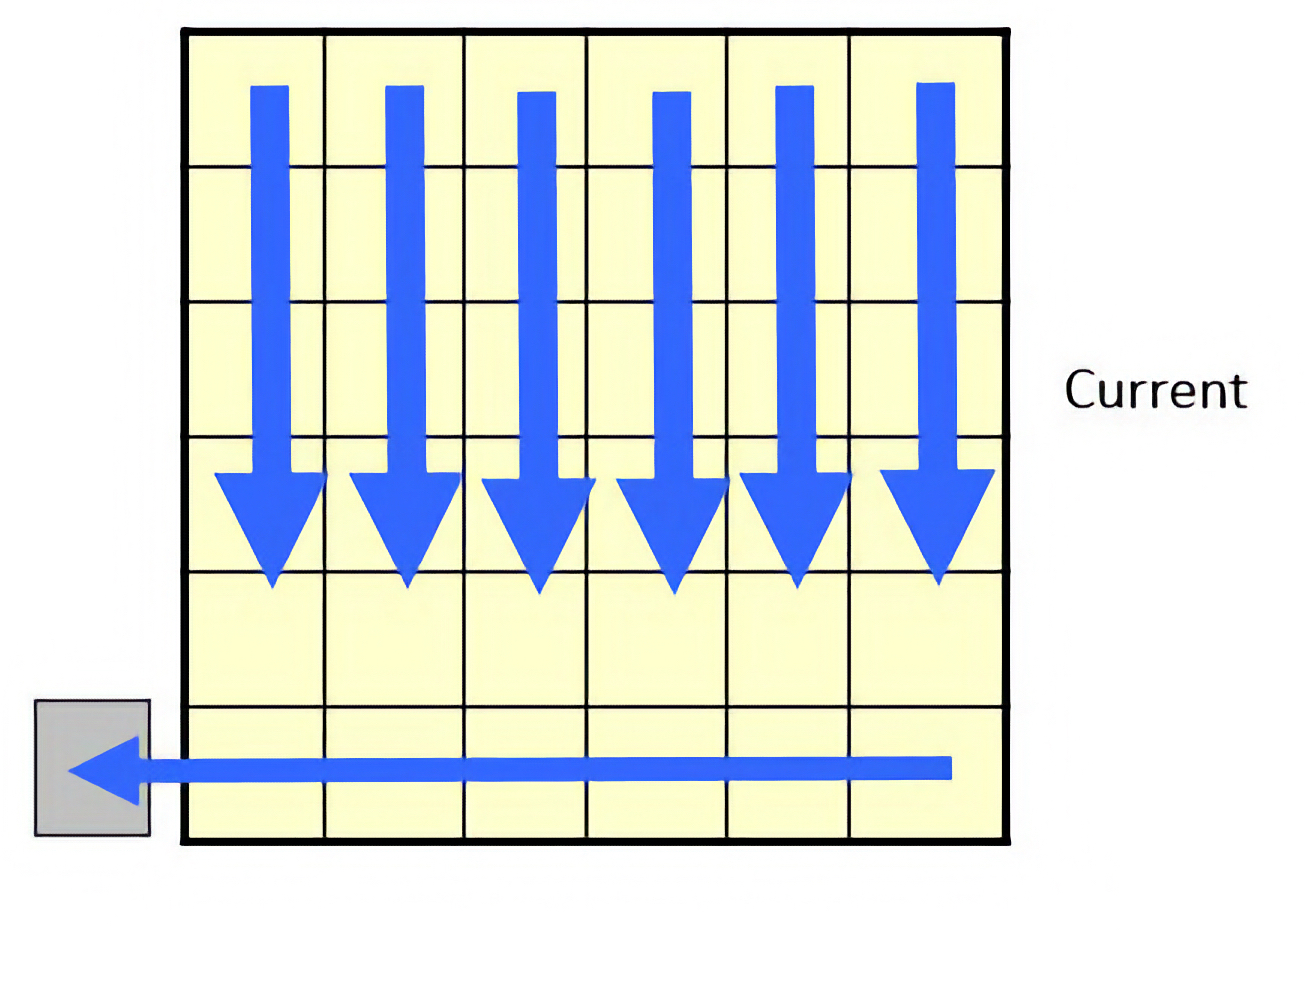
\includegraphics[width=0.7\textwidth]{3.Conceptos_Previos/CCD.jpg}
    \caption{Diagrama de funcionamiento de un sensor CCD.\\ Fuente: \cite{ccd_operation_diagram}.}
    \label{fig:CCD}
\end{figure}

Los sensores CCD (Dispositivo de Carga Acoplada) han sido durante años el estándar en misiones de observación espacial, gracias a su excelente calidad de imagen y desempeño en condiciones de baja iluminación. Funcionan acumulando carga en pozos de potencial dentro de un sustrato semiconductor, transfiriendo luego estas cargas secuencialmente a un nodo de salida para su lectura.

Destacan por su amplio rango dinámico, que puede duplicar al de los CMOS, y su bajo ruido de lectura, ideal para observaciones nocturnas o en bandas espectrales de baja radiancia. Presentan una notable uniformidad entre píxeles, reduciendo el ruido de patrón fijo y facilitando la calibración radiométrica. Además, al tener menos electrónica integrada en cada píxel, ofrecen un mayor factor de llenado, aprovechando mejor el área fotosensible.

Como aspectos menos favorables, presentan un consumo energético elevado, lo que puede ser un inconveniente en plataformas con recursos limitados. La dependencia de electrónica externa incrementa volumen y masa del sistema. También pueden sufrir el efecto \textit{blooming}, donde un píxel saturado afecta a los adyacentes, y su velocidad de lectura, relativamente baja, restringe su capacidad para captar escenas dinámicas. Asimismo, su sensibilidad a la radiación espacial puede degradar su rendimiento en misiones prolongadas \cite{kuroda_essential_2014}.

\subsubsection{Sensores CMOS (Complementary Metal-Oxide Semiconductor)}

\begin{figure}[H]
    \centering
    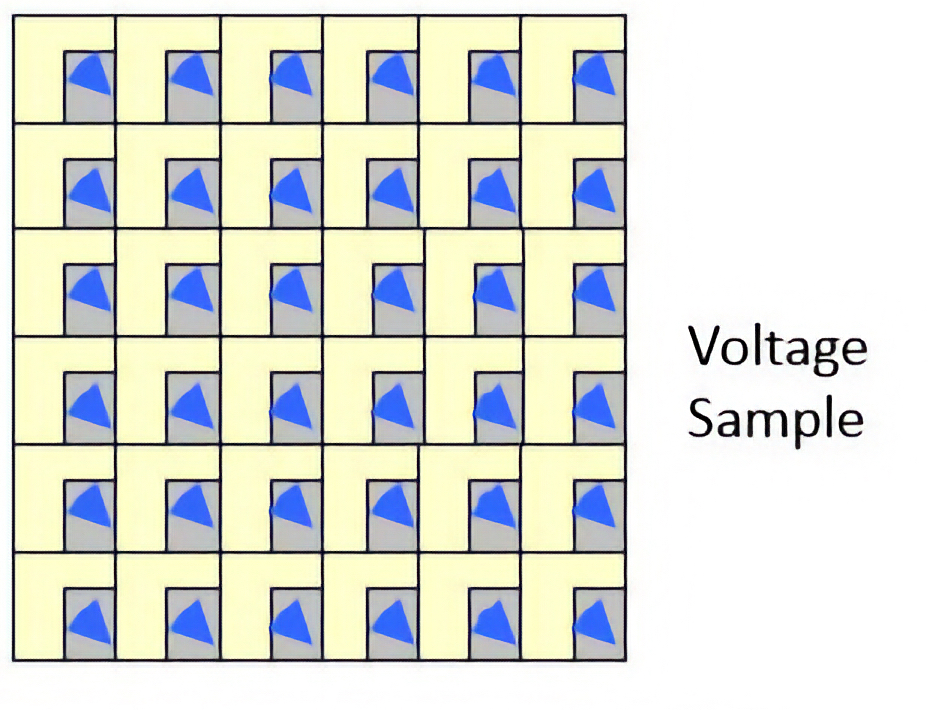
\includegraphics[width=0.7\textwidth]{3.Conceptos_Previos/CMOS.jpg}
    \caption{Diagrama de funcionamiento de un sensor CMOS.\\Fuente: \cite{ccd_operation_diagram}.}
    \label{fig:CMOS}
\end{figure}
Los sensores CMOS han ganado protagonismo en aplicaciones espaciales en los últimos años, debido a sus ventajas operativas en entornos con restricciones de recursos. A diferencia de los CCD, los CMOS integran circuitos de amplificación y procesamiento en cada píxel, permitiendo lecturas directas y selectivas.

Entre sus ventajas sobresalen su bajo consumo energético, típicamente entre una décima y una centésima parte del de un CCD comparable. Permiten lecturas parciales a alta velocidad, facilitando modos operativos flexibles, y su integración de funciones adicionales en el chip simplifica los sistemas, reduciendo su masa. También presentan una mayor tolerancia a la radiación, lo que los hace atractivos para misiones prolongadas.

Como desafíos, los primeros sensores CMOS mostraban mayores niveles de ruido de lectura y ruido de patrón fijo, aunque los desarrollos recientes han mitigado estas diferencias. El menor factor de llenado, debido a la electrónica en cada píxel, se compensa actualmente con microlentes que concentran la luz. Otro aspecto a considerar es el fenómeno \textit{rolling shutter}, que puede distorsionar imágenes con objetos en rápido movimiento, aunque las versiones con \textit{global shutter} resuelven este inconveniente. Finalmente, su sensibilidad en condiciones de baja iluminación, anteriormente inferior a la de los CCD, ha mejorado considerablemente con las tecnologías retroiluminadas \cite{kuroda_essential_2014}.

\subsubsection{Sensores HgCdTe}

\begin{figure}[H]
    \centering
    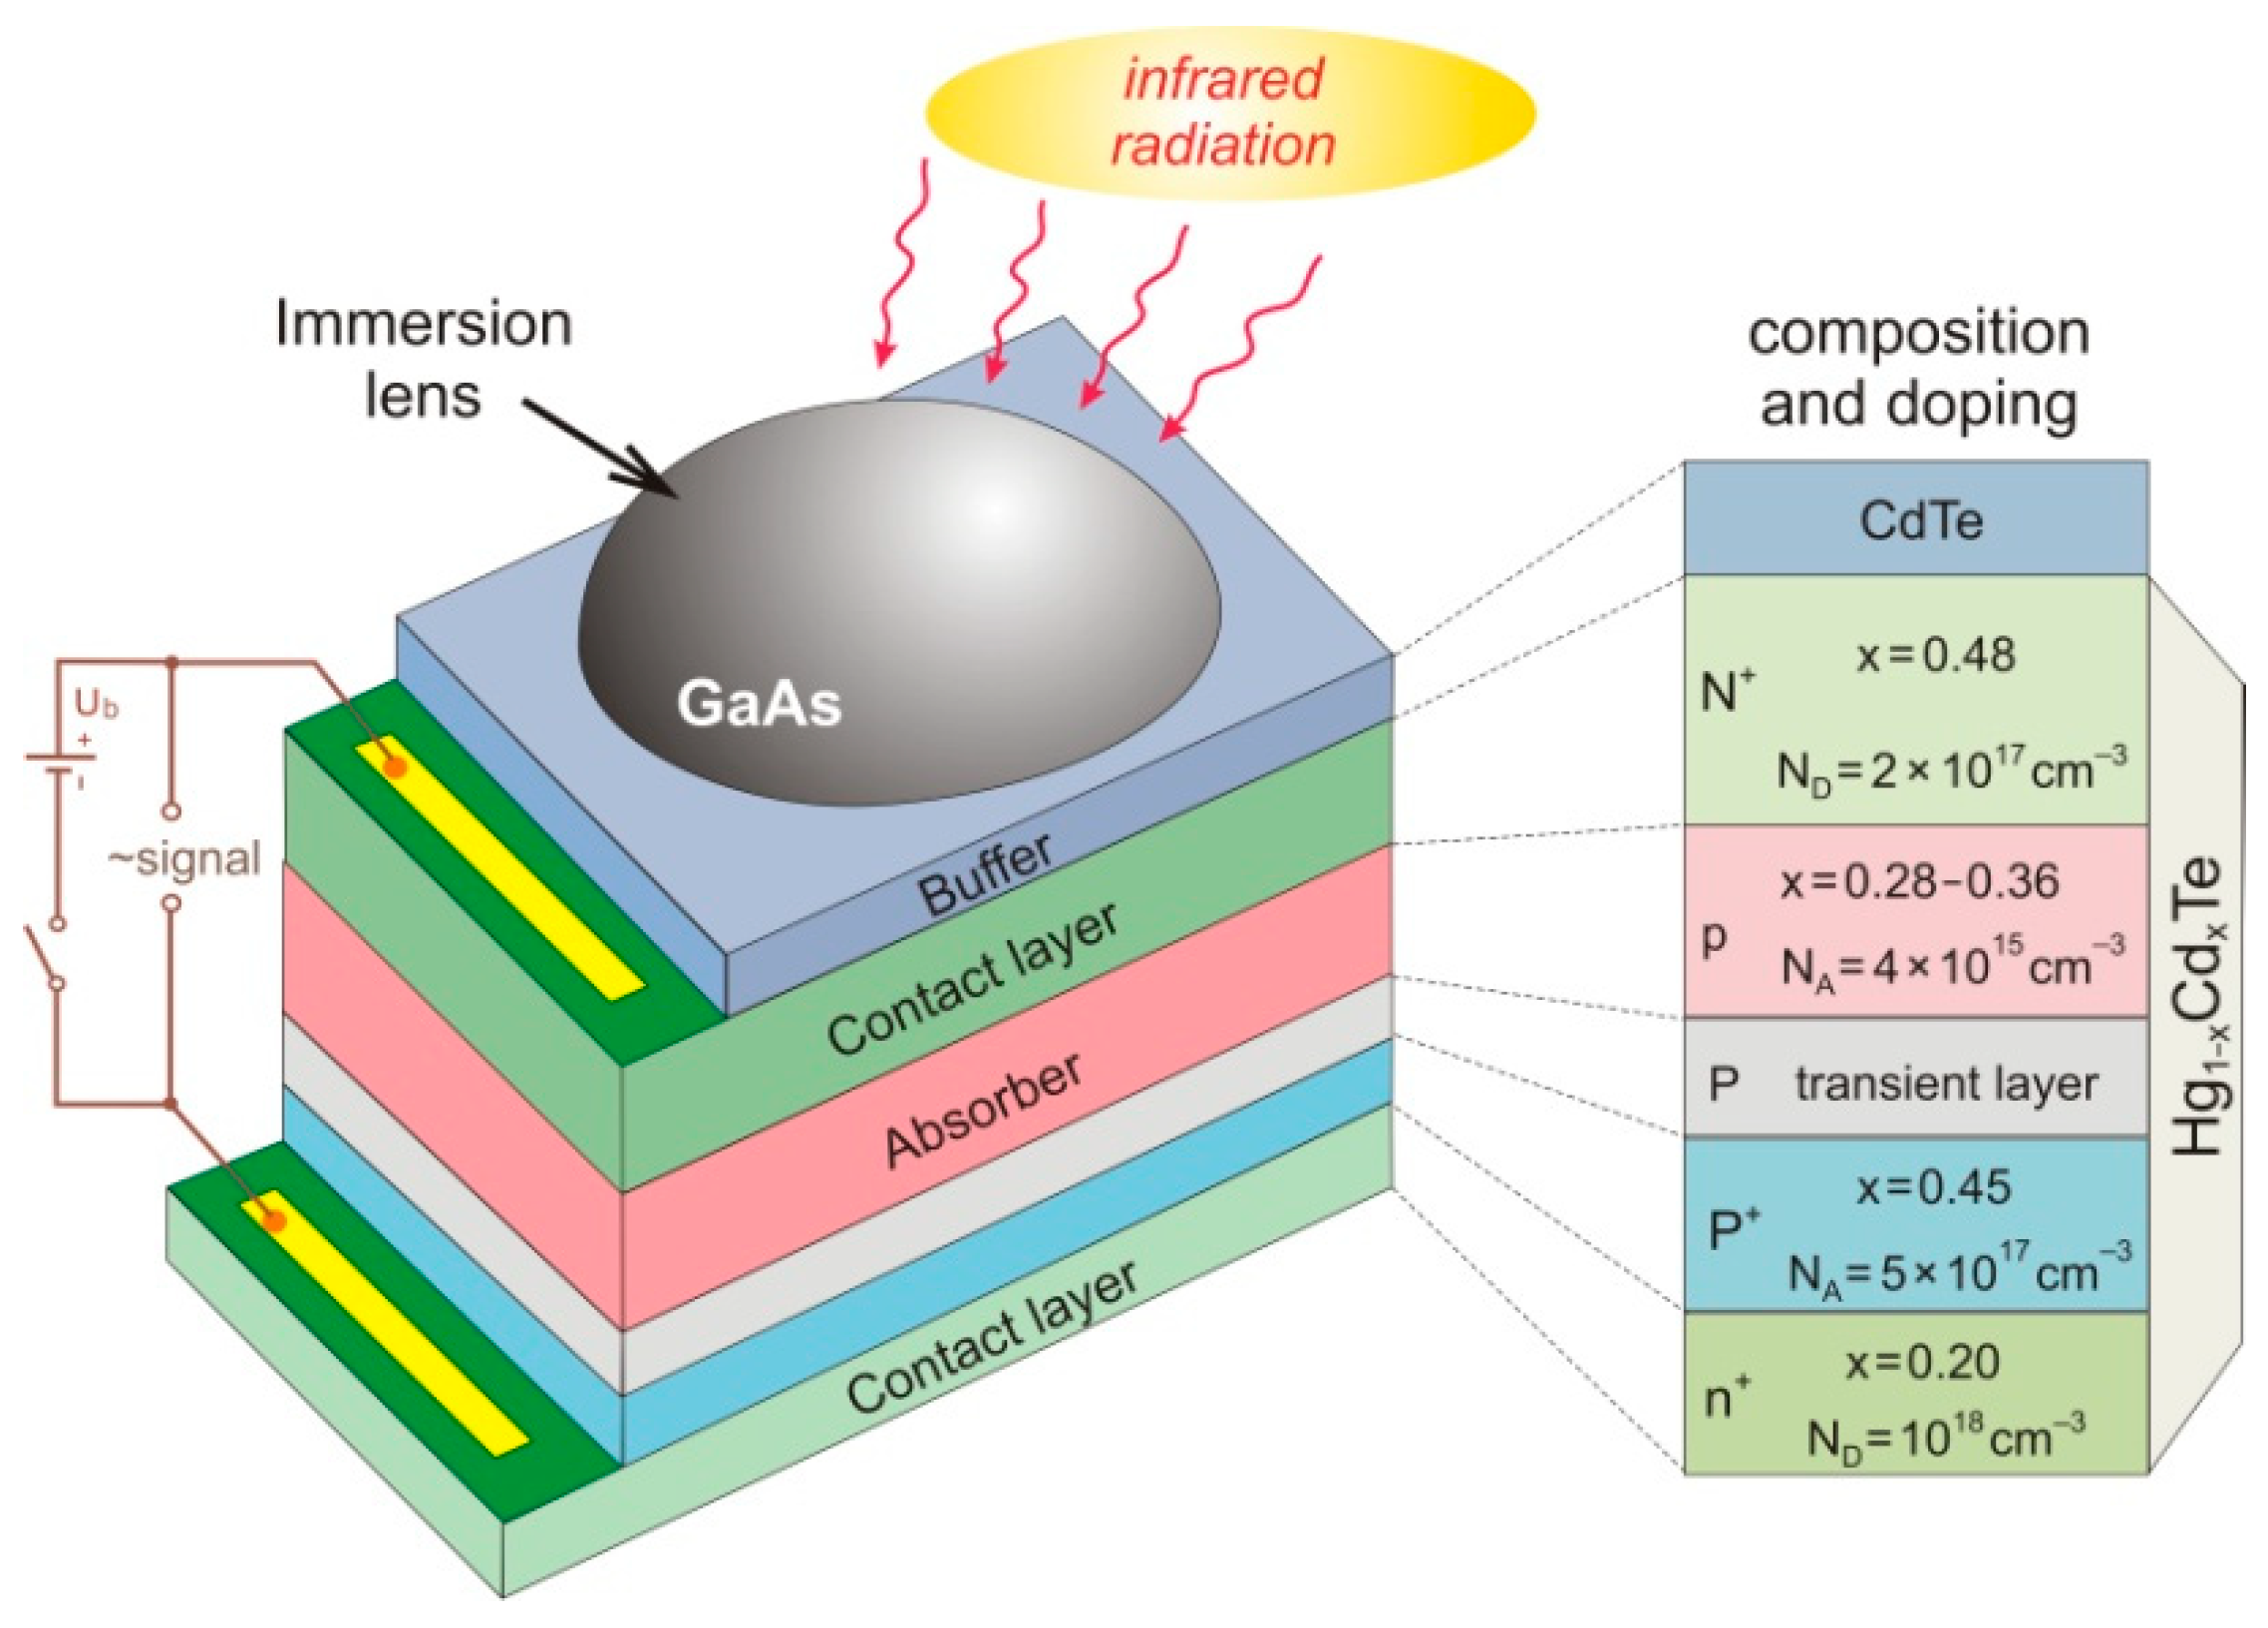
\includegraphics[width=0.5\linewidth]{3.Conceptos_Previos/coatings-11-00611-g002-2725805712.png}
    \caption{Disposición del detector MCT.\\Fuente: \cite{coatings2021_11_5_611_extended}.}
    \label{fig:enter-label}
\end{figure}

Los sensores de telururo de mercurio y cadmio (abreviado como MCT o HgCdTe) son reconocidos por su versatilidad espectral, con un rango ajustable entre 1 y 30 \textmu m mediante variaciones en la composición de la aleación. Esta adaptabilidad, unida a una eficiencia cuántica excepcional y tiempos de respuesta en nanosegundos, los posiciona como estándar en aplicaciones críticas como imágenes térmicas militares, astronomía infrarroja y detección de gases. Sus ventajas incluyen la capacidad de operar en modos fotoconductivo y fotovoltaico, alta detectividad incluso a temperaturas cercanas a ambiente y la posibilidad de crear estructuras de banda prohibida graduada para optimizar la absorción de fotones. Sin embargo, enfrentan desafíos como la toxicidad intrínseca del mercurio, que complica su fabricación y disposición final, y la sensibilidad a defectos cristalográficos durante el crecimiento epitaxial, lo que eleva los costos y reduce el rendimiento en dispositivos de gran área. Además, requieren sistemas de enfriamiento avanzados (criogénicos o mediante efecto Peltier) para minimizar el ruido térmico en aplicaciones de alta precisión, incrementando la complejidad del sistema global. A pesar de esto, siguen siendo insustituibles en aplicaciones que exigen cobertura espectral amplia y gran resolución térmica \cite{capper_mercury_2010}.

\subsubsection{Sensores InGaAs}


\begin{figure}[H]
    \centering
    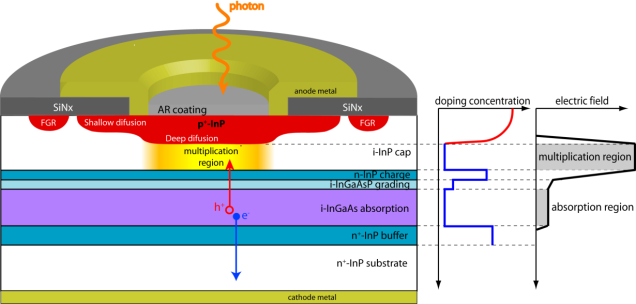
\includegraphics[width=0.5\linewidth]{3.Conceptos_Previos/ingaas_cross-1213932152.png}
    \caption{Disposición de capas típica del detector InGaAs. \\Fuente: \cite{everyphotoncounts2025ingaas_spad}.}
    \label{fig:enter-label}
\end{figure}

Los sensores de arseniuro de galio e indio (InGaAs) destacan por su capacidad para detectar radiación en el infrarrojo cercano (NIR), con un rango espectral típico entre 0,9 y 1,7 \textmu m, extendible hasta 2,55 \textmu m en versiones especializadas. Su estructura híbrida combina fotodiodos de InGaAs con circuitos CMOS, aprovechando una alta eficiencia cuántica y baja corriente oscura, lo que los hace ideales para aplicaciones que requieren precisión en condiciones de baja luminosidad. Entre sus ventajas destacan la sensibilidad extendida en el NIR, la capacidad de operar con requisitos de enfriamiento moderados y la ausencia de materiales tóxicos como el mercurio o el cadmio, cumpliendo con regulaciones ambientales. No obstante, presentan limitaciones como un ruido de corriente oscura significativo en entornos de alta temperatura, costos elevados debido a los procesos de fabricación complejos y fragilidad mecánica que exige manipulación cuidadosa. Además, su rendimiento en longitudes de onda superiores a 2 \textmu m tradicionalmente ha sido inferior al de otras tecnologías, aunque avances recientes están mitigando esta brecha \cite{henini_handbook_2002}.


\subsection{\textit{Time Delay and Integration} (TDI)}\label{sec:tdi}

\begin{figure}[H]
    \centering
    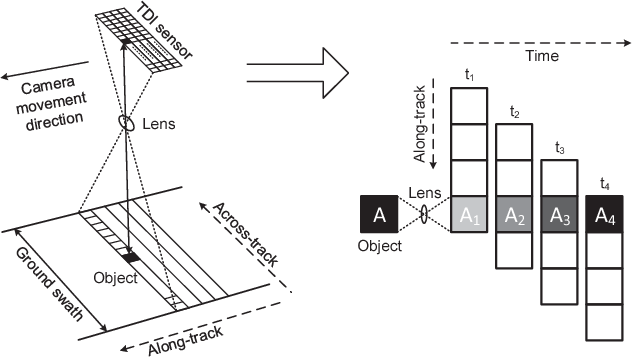
\includegraphics[width=0.7\textwidth]{3.Conceptos_Previos/TDI.png}
    \caption{Esquema de funcionamiento del \textit{Time Delay Integration}.\\Fuente: \cite{tdi_sensor2017}.}
    \label{fig:TDI}
\end{figure}

El TDI permite aumentar el tiempo efectivo de exposición sin desenfoque por movimiento, mejorando la relación señal-ruido en condiciones de baja iluminación o cuando se requieren tiempos de integración cortos debido a la velocidad de desplazamiento\cite{design_workshop_optical_2023}.

Consiste en una serie de líneas de píxeles que capturan sucesivamente la misma escena, desplazando la carga generada de una línea a otra en sincronía con el movimiento de la imagen sobre el detector. Esto permite acumular la carga correspondiente a un mismo punto a lo largo de varias etapas, aumentando efectivamente el tiempo de exposición.

Esta técnica exige una sincronización precisa entre la velocidad de transferencia de carga y la velocidad de desplazamiento de la imagen proyectada. Cualquier desajuste afectaría la resolución espacial, provocando desenfoque. Al multiplicar el tiempo de exposición por el número de etapas, permite mejorar notablemente la sensibilidad sin sacrificar resolución espacial.


\subsection{Estrategias de Escaneo en Sistemas de Observación Satelital}

Para adquirir imágenes de la superficie terrestre desde una órbita, resulta indispensable definir una estrategia de escaneo que permita cubrir progresivamente la zona de interés. Estas estrategias determinan cómo se captura la información espacial y temporalmente, considerando tanto la configuración del detector como el movimiento relativo entre el satélite y la superficie terrestre. A continuación, se describen las principales técnicas empleadas en sistemas de observación orbital, junto con sus ventajas, limitaciones y ámbitos de aplicación característicos\cite{design_workshop_optical_2023}.


\subsubsection{Tecnología Pushbroom (Barrido Lineal)}

\begin{figure}[H]
    \centering
    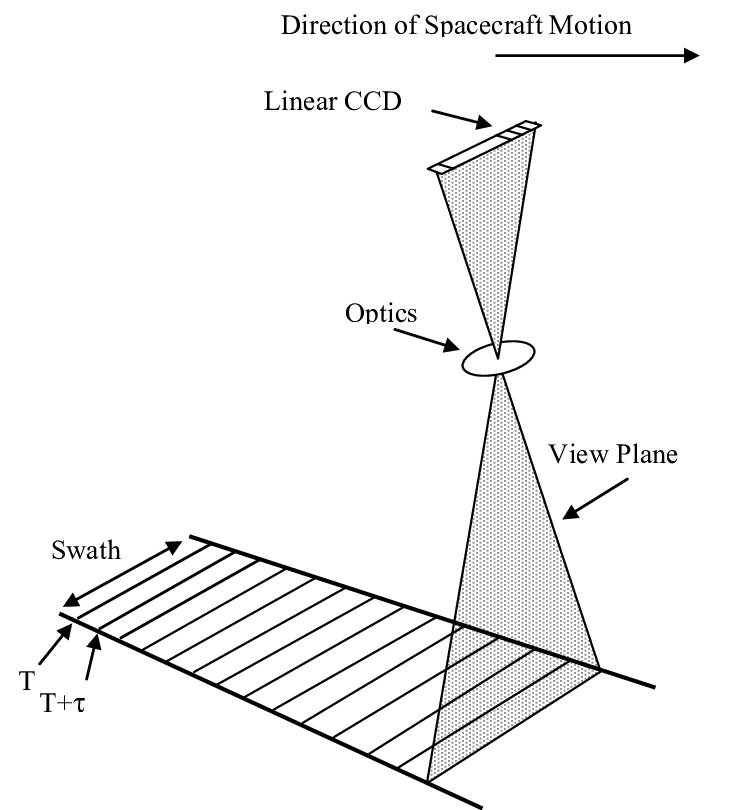
\includegraphics[width=0.7\textwidth]{3.Conceptos_Previos/Pushbroom.png}
    \caption{Funcionamiento del escaneo \textit{Pushbroom}.\\Fuente: \cite{pushbroom_sensor_diagram}.}
    \label{fig:Pushbroom}
\end{figure}


La tecnología Pushbroom es una de las más utilizadas actualmente en observación terrestre desde satélites. Utiliza una línea de detectores dispuestos perpendicularmente a la dirección de vuelo. Esta línea captura simultáneamente una franja del terreno, mientras que el movimiento orbital permite generar la imagen completa.

Sus ventajas incluyen una mayor relación señal-ruido gracias al tiempo de observación más prolongado sobre cada punto y la ausencia de componentes mecánicos móviles, lo que aumenta su fiabilidad. Como desafío, presenta variaciones en la sensibilidad entre detectores individuales que pueden provocar franjas si no se calibra adecuadamente. Además, suele ofrecer una resolución espacial ligeramente inferior a los escáneres Whiskbroom para un mismo ancho de barrido.

\subsubsection{Tecnología Whiskbroom (Barrido Transversal)}

\begin{figure}[H]
    \centering
    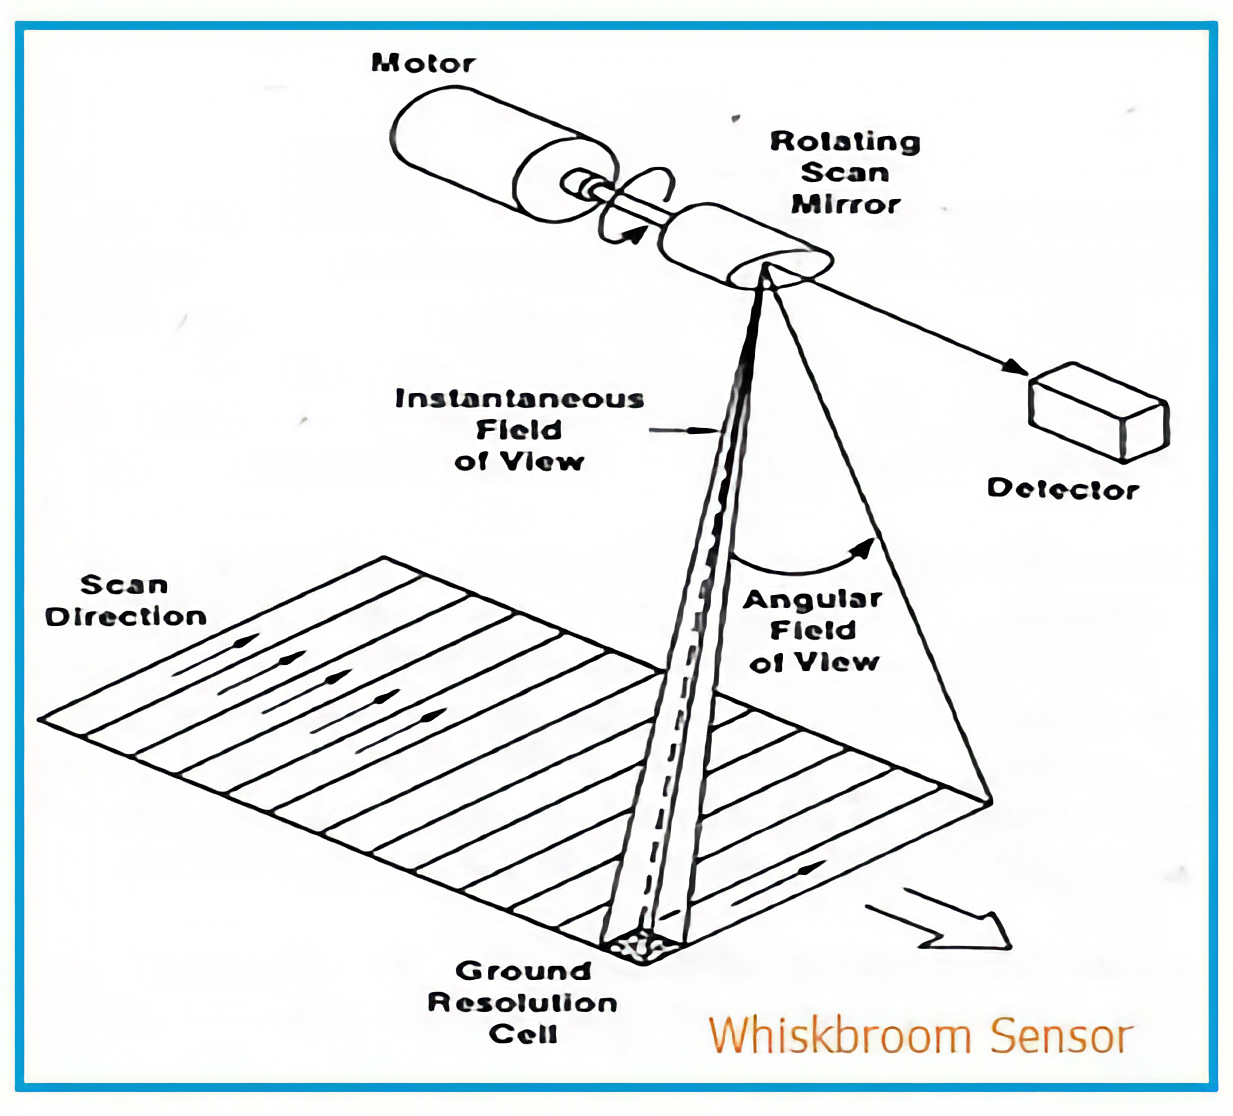
\includegraphics[width=0.7\textwidth]{3.Conceptos_Previos/whiskbroom.jpg}
    \caption{Funcionamiento del escaneo \textit{Whiskbroom}.\\Fuente: \cite{whiskbroom_diagram}.}
    \label{fig:whiskbroom}
\end{figure}

Los escáneres Whiskbroom funcionan mediante un espejo oscilante que barre perpendicularmente a la trayectoria del satélite, dirigiendo la luz hacia uno o pocos detectores.

Su principal ventaja es la alta resolución espacial alcanzable, ya que permite concentrar la observación en pequeñas áreas mediante un número reducido de detectores, facilitando la uniformidad radiométrica. Como contrapartida, incorporan componentes mecánicos móviles que aumentan el peso y la complejidad, y su menor tiempo de observación por píxel limita su sensibilidad en condiciones de baja iluminación. Además, su naturaleza secuencial restringe la velocidad máxima de adquisición.

\subsubsection{Enfoque Step-Stare (Configuración de Imagen Estática)}

\begin{figure}[H]
    \centering
    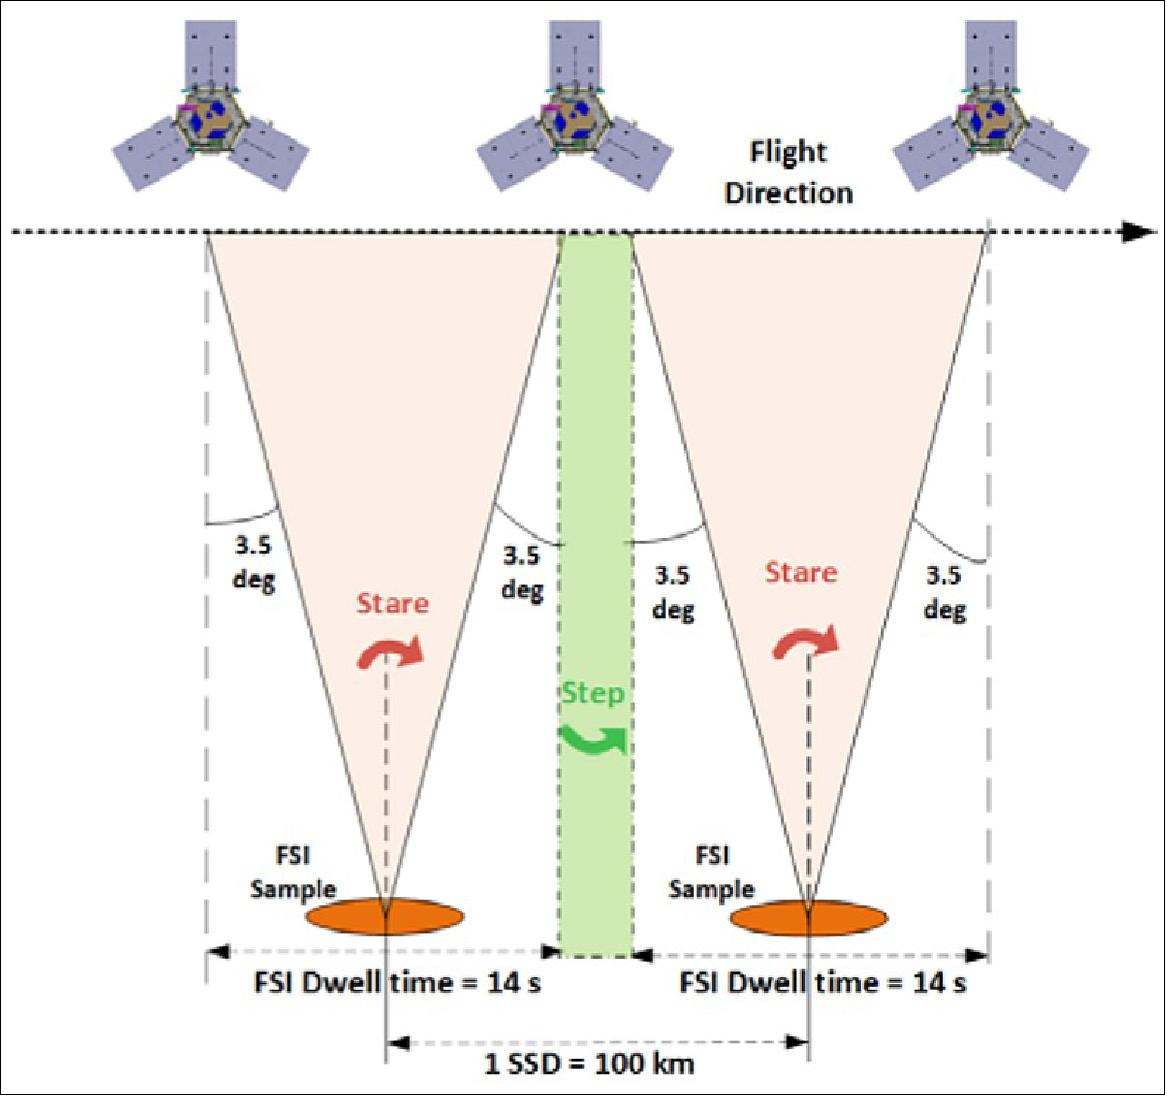
\includegraphics[width=0.7\textwidth]{3.Conceptos_Previos/Step Stare.jpeg}
    \caption{Funcionamiento del escaneo \textit{Step-Stare}.\\Fuente: \cite{step_stare_system}.}
    \label{fig:Stepstare}
\end{figure}

El enfoque Step-Stare captura imágenes bidimensionales completas de forma discreta, similar a una cámara fotográfica. Entre exposiciones, el sistema óptico se reorienta hacia la siguiente área de interés.

Esta configuración maximiza la eficiencia en la recolección de fotones al dedicar todo el tiempo de exposición a cada imagen, logrando excelente relación señal-ruido. Permite también apuntamiento flexible, ideal para monitoreo de emergencias o eventos dinámicos. Como aspectos a considerar, requiere compensar el movimiento de la plataforma para evitar desenfoque y presenta menor eficiencia en la cobertura continua de grandes áreas, debido al tiempo adicional necesario para reposicionar el sistema entre capturas.

\subsection{Disposición de detectores}

En el diseño del plano focal para la carga útil óptica, la disposición de los detectores es un aspecto clave que afecta tanto la calidad de imagen como la viabilidad técnica y económica del satélite. Existen varias estrategias para el \textit{layout} de detectores, entre las que destacan \cite{kaplan_optical_2011}:

\begin{itemize}
    \item \textbf{Divisores de campo (Divoli o \textit{Field Splitters})}: Esta solución emplea elementos ópticos para dividir el campo de visión en regiones independientes, cada una dirigida a un detector específico. Permite optimizar la captación de diferentes bandas espectrales o maximizar el área cubierta por cada detector, facilitando la especialización de cada canal detector para una banda concreta o para mejorar la redundancia y la relación señal/ruido (SNR) en segmentos críticos del espectro.

    \item \textbf{Divisores de haz (\textit{Beam Splitters})}: Utilizados para separar la luz en distintas longitudes de onda y redirigirlas a detectores diferentes. Esta técnica es útil cuando se requieren bandas espectrales muy diferenciadas, aunque introduce pérdidas ópticas y puede complicar el alineamiento y la calibración radiométrica.

    \item \textbf{Solapamiento parcial de detectores}: En algunos diseños, se solapan parcialmente las áreas sensibles de los detectores para mejorar la corregistración entre bandas o aumentar la redundancia. Sin embargo, esto incrementa la complejidad del procesamiento y puede penalizar la eficiencia espacial y el peso del sistema.
\end{itemize}

A la hora de dimensionar la misión, se establece un límite máximo de \textbf{tres detectores}, con el fin de simplificar la disposición de los mismos \cite{design_workshop_optical_2023}.

\section{Óptica. Telescopios}

La óptica de un satélite de observación es el conjunto de elementos (lentes, espejos, filtros, etc.) que recogen la radiación electromagnética proveniente de la Tierra y la enfocan sobre el detector. El telescopio es el corazón de este sistema óptico: su función es formar una imagen nítida y de alta calidad sobre el plano focal, maximizando la resolución espacial y la eficiencia de captación de luz, minimizando aberraciones y pérdidas de contraste.
La elección del tipo de telescopio depende de los requisitos de la misión (resolución, campo de visión, peso, facilidad de alineamiento y fabricación, etc.). Los diseños más usados en teledetección espacial son los telescopios refractivos y los reflectores de dos o tres espejos (Cassegrain, Korsch, TMA) \cite{design_workshop_optical_2023}.

\subsection{Parámetros ópticos relevantes}

\begin{figure}[H]
    \centering
    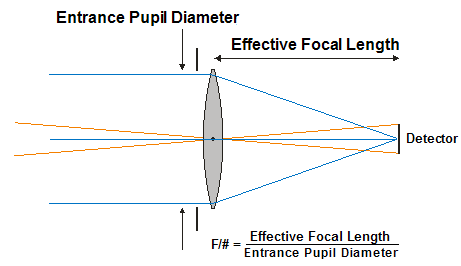
\includegraphics[width=0.7\textwidth]{3.Conceptos_Previos/eoirOptical1.png}
    \caption{Diagrama de parámetros ópticos. \\Fuente: \cite{entrance_pupil_diagram}.}
    \label{fig:Lente}
\end{figure}

\subsubsection*{Diámetro de pupila ($D$)}

El diámetro de pupila es el tamaño de la apertura circular por la que entra la luz al sistema óptico, también conocido como apertura del telescopio. Este parámetro es crucial porque determina la cantidad de luz que puede captar el sistema (afectando a la SNR) y el límite de difracción, es decir, la máxima resolución teórica que puede alcanzar el instrumento. Un mayor diámetro de pupila permite captar más luz y obtener una mejor resolución espacial, pero también incrementa el peso y el tamaño del instrumento, lo que es crítico en satélites donde se busca minimizar la masa para reducir costes de lanzamiento.

\subsubsection*{Distancia focal ($f$)}

La distancia focal es la separación entre el centro óptico del sistema (o el espejo principal, en sistemas reflectores) y el plano focal donde se forma la imagen. Este parámetro define el aumento del sistema: a mayor distancia focal, mayor es la imagen proyectada sobre el detector para un mismo objeto observado en la Tierra. En instrumentos de observación, la distancia focal se elige para cumplir con el GSD requerido, ya que está relacionada con el tamaño del píxel del detector y la resolución en superficie.

\subsubsection*{Relación focal ($F\#$)}

La relación focal se define como el cociente entre la distancia focal y el diámetro de pupila ($F\#=\frac{f}{D}$). Para los sistemas obscurados, se define la relación focal equivalente $T\#$, que viene dada por la relación:
\begin{align}
\label{relfoc}
    T\# = \frac{f}{\sqrt{D^2(1-R_{obs}^2)}} 
\end{align}

Siendo $R_{obs}$ la misma relación de obscuración en la ecuación \ref{mtfrobs}
Es un parámetro clave ya que in número $F\#$ bajo (óptica “rápida”) implica una apertura grande respecto a la distancia focal, lo que permite captar más luz y mejora la SNR, pero puede aumentar las aberraciones ópticas y reducir la profundidad de campo. Un número $F\#$ alto (óptica “lenta”) reduce la cantidad de luz captada, pero suele simplificar el diseño y controlar mejor las aberraciones. La relación focal afecta directamente a la MTF, la SNR y la saturación del detector.


\subsection{Tipos de telescopio}


\subsubsection{Refractivo}

\begin{figure}[H]
    \centering
    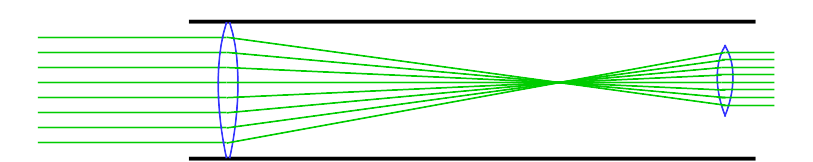
\includegraphics[width=0.7\textwidth]{3.Conceptos_Previos/refractor-vs-reflector-4239218127.png}
    \caption{Telescopio Refractivo. \\ Fuente: \cite{refractor_reflector_comparison}.}
    \label{fig:Refractive}
\end{figure}

El telescopio refractivo utiliza lentes para enfocar la luz sobre el detector. Su principal ventaja es la ausencia de obscuración, ya que toda la apertura está disponible para captar luz. Esto se traduce en una MTF de difracción más alta, especialmente a frecuencias espaciales elevadas, y en una penalización por alineamiento relativamente baja ($MTF_{alineamiento} \approx 0,90$), pues el sistema es sencillo de montar y ajustar. Sin embargo, los telescopios refractivos presentan aberraciones cromáticas, lo que limita su uso en aplicaciones multiespectrales o en longitudes de onda fuera del visible. Además, para grandes aperturas (entre 80 y 100 mm), las lentes se vuelven pesadas y difíciles de fabricar, lo que desincentiva su uso en satélites de observación de alta resolución, o de orbitas mayores a LEO (\textit{Low Earth Orbit}).


\subsubsection{Cassegrain}

\begin{figure}[H]
    \centering
    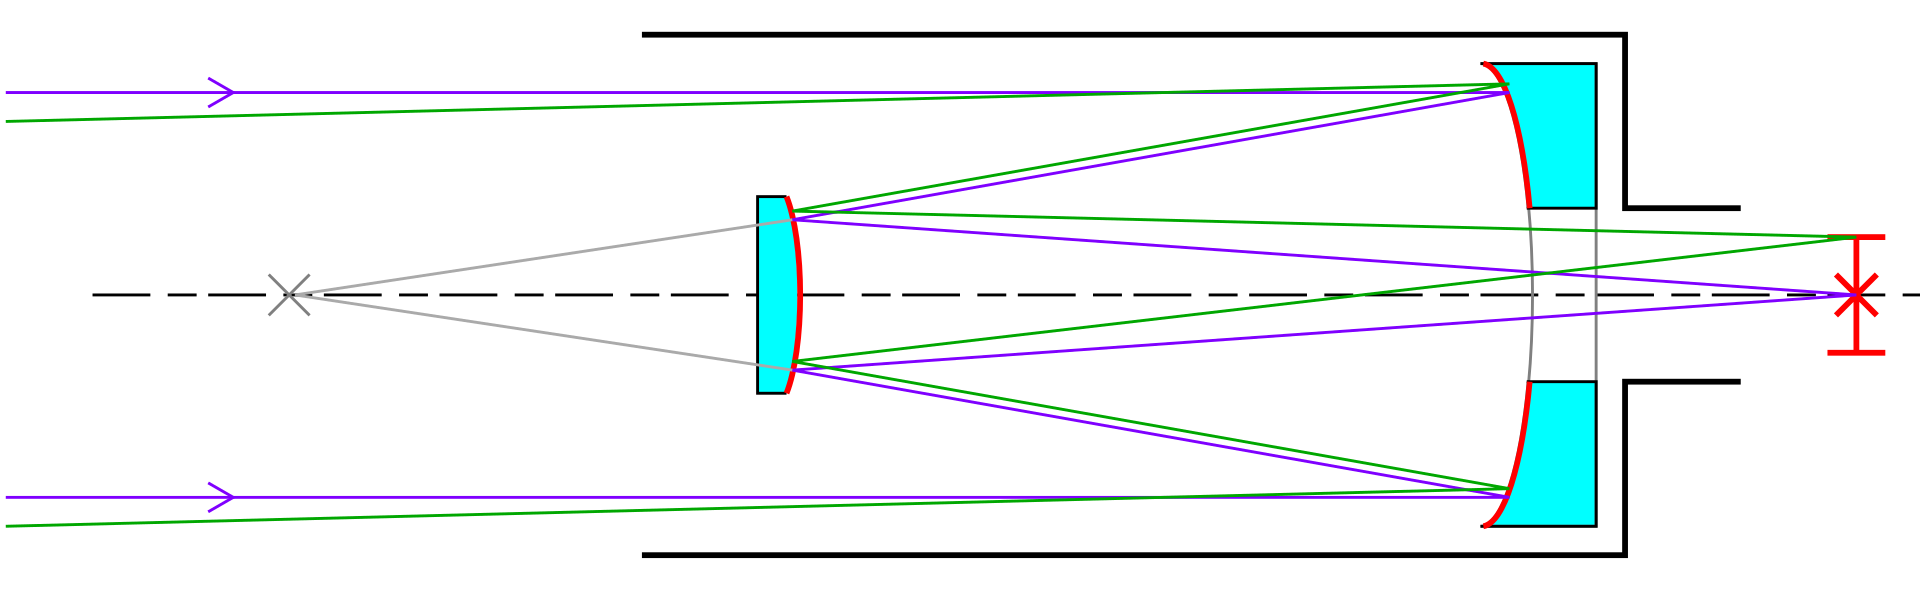
\includegraphics[width=0.7\textwidth]{3.Conceptos_Previos/Cassegrain_Telescope.svg.png}
    \caption{Telescopio Cassegrain. \\Fuente: \cite{cassegrain_telescope_diagram}.}
    \label{fig:Cassegrain}
\end{figure}

El diseño Cassegrain es un reflector de dos espejos, con un primario parabólico y un secundario hiperbólico. La luz se refleja primero en el espejo primario, luego en el secundario y finalmente pasa a través de un orificio en el primario hacia el detector. Este sistema introduce una obscuración central debida al secundario, lo que reduce la MTF de difracción a frecuencias altas, pero permite una configuración compacta y una buena corrección de aberraciones cromáticas. El alineamiento es moderadamente sencillo, con una penalización típica de $MTF_{alineamiento} \approx 0,85$. El campo de visión es limitado, típicamente en torno a 3°.

\subsubsection{Korsch}

\begin{figure}[H]
    \centering
    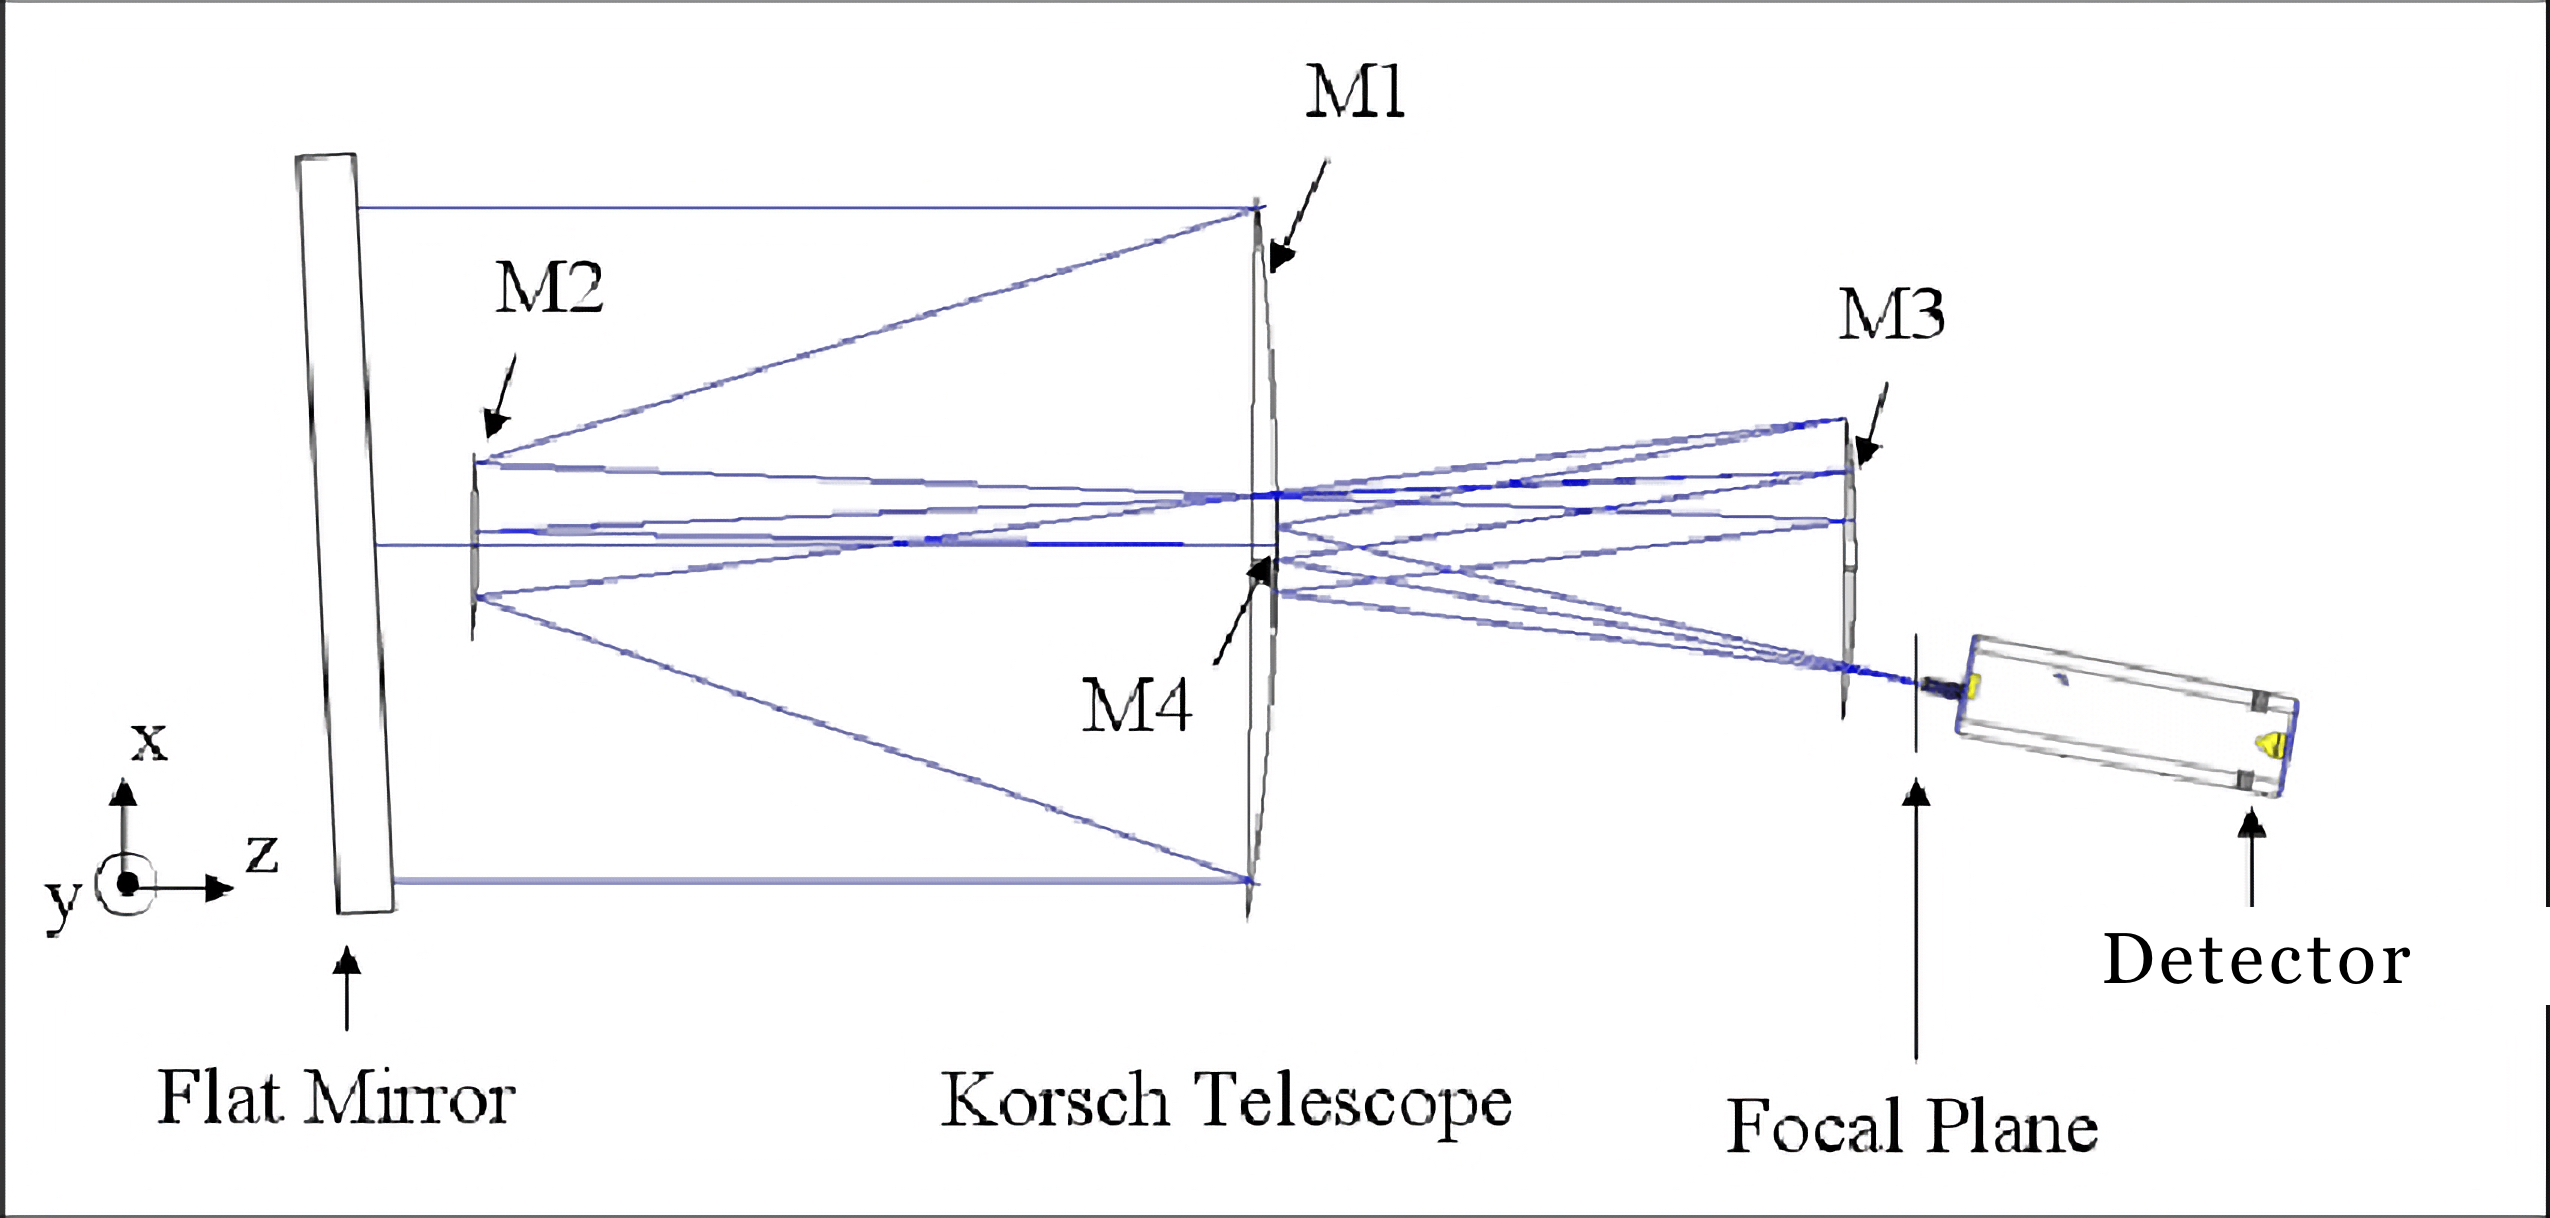
\includegraphics[width=0.7\textwidth]{3.Conceptos_Previos/Korsch.jpg}
    \caption{Telescopio Korsch. \\Fuente: \cite{korsch_telescope_system}.}
    \label{fig:Korsch}
\end{figure}

El telescopio Korsch es un reflector de tres espejos, también con obscuración central. Su diseño está optimizado para controlar la luz parásita (straylight). Permite focales largas y una buena calidad de imagen en todo el campo, aunque el alineamiento es más complejo y la penalización en la MTF por este motivo es mayor ($MTF_{alineamiento} \approx 0,80$). La presencia de la obscuración central sigue penalizando la MTF de difracción, aunque el control de aberraciones es excelente. Posee un FoV similar al Cassegrain, de $3º$.

\subsubsection{\textit{Three-mirror anastigmat} (TMA)}

\begin{figure}[H]
    \centering
    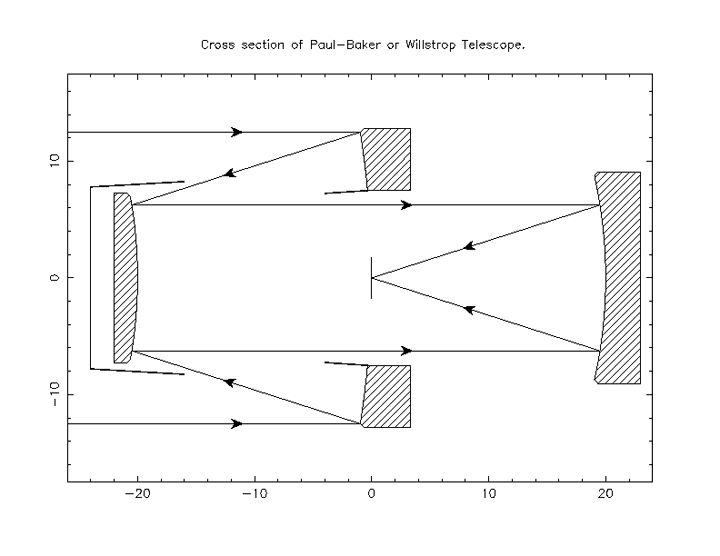
\includegraphics[width=0.7\textwidth]{3.Conceptos_Previos/TMA.png}
    \caption{Telescopio TMA. \\Fuente: \cite{tma_telescope_diagram}.}
    \label{fig:Tma}
\end{figure}

El telescopio de tres espejos anastigmático es un reflector de tres espejos sin obscuración central, ya que el haz óptico se desvía fuera del eje óptico principal (diseño off-axis). Esto permite un campo de visión mas amplio, del orden de $8º$, y una calidad de imagen homogénea en todo el campo, sin penalización por la presencia de elementos que bloqueen la apertura. Sin embargo, el alineamiento de un TMA es extremadamente exigente, con una penalización en la MTF de alineamiento significativa ($MTF_{alineamiento} \approx 0,70$). Además, la fabricación y verificación de estos sistemas es más compleja y costosa.

\subsubsection*{Tabla comparativa de Telescopios}

\begin{table}[H]
\caption{Comparativa de tipos de sistemas ópticos.}
\centering
\begin{tabular}{l c c c c}
\hline
\textbf{Tipo} & \textbf{Obscuración($R_{obs}$)} & \textbf{$FoV_{lim}$} & \textbf{MTF\textsubscript{Alineamiento}} & \textbf{Transmisión óptica $(\tau)$} \\
\hline
Refractivo\tablefootnote{ Limitado a 80 mm de diámetro máximo válido para el presente trabajo}    & No  & 10º & 0,90 & 0,8 \\
Cassegrain    & Sí (0,2)  & 3º  & 0,85 & 0,7 \\
Korsch        & Sí (0,2)  & 3º  & 0,80 & 0,65 \\
TMA           & No  & 8º  & 0.70 & 0,6 \\
\hline
\end{tabular}

\label{tab:tabla_telescopios}
\end{table}



\subsection{Filtros}

\begin{figure}[H]
    \centering
    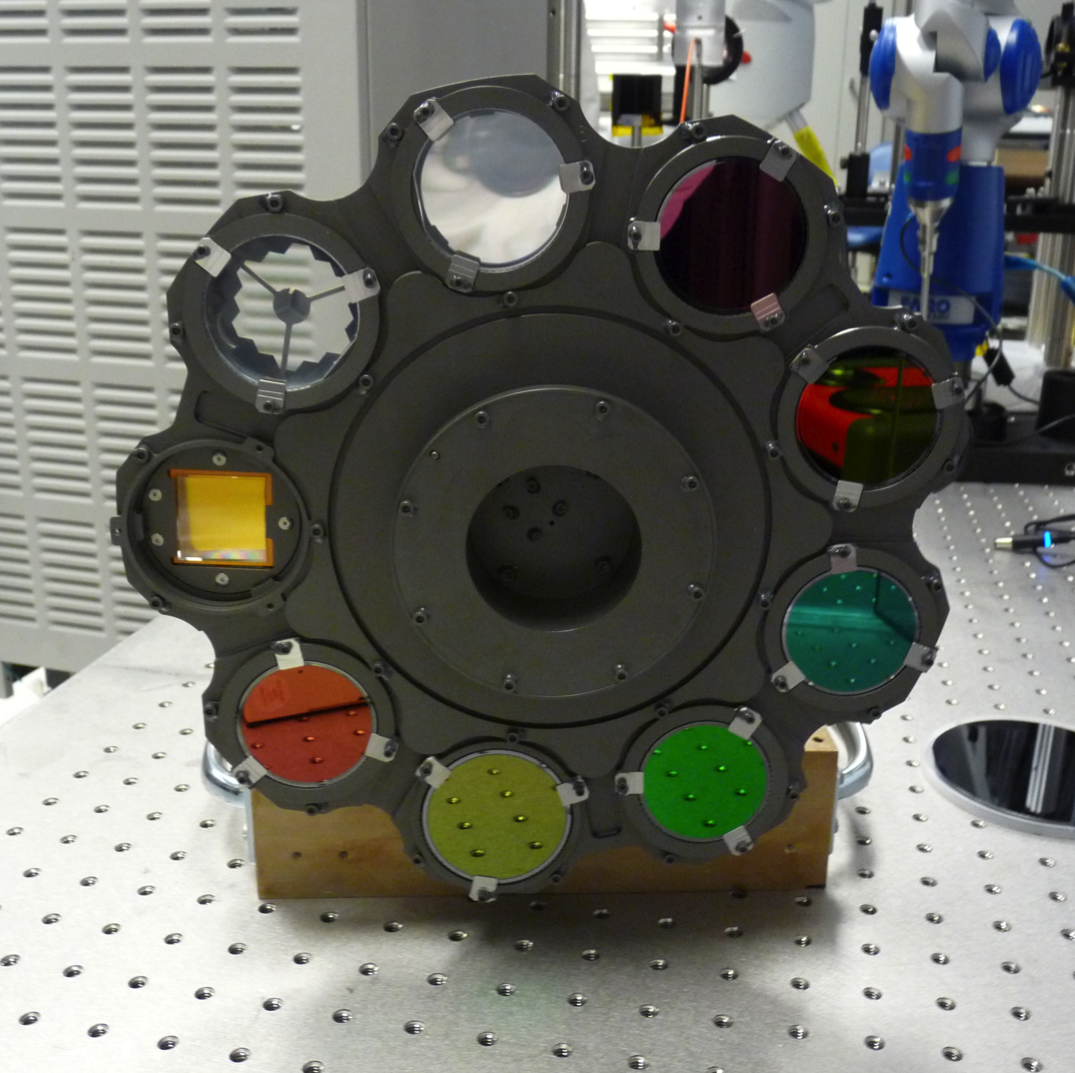
\includegraphics[width=0.7\textwidth]{3.Conceptos_Previos/NIRISS_FilterWheel.png}
    \caption{Rueda de Filtros del \textit{James Webb Space Telescope}. \\Fuente: \cite{STScI_MIRI_Filters}.}
    \label{fig:Filter}
\end{figure}

La selección de filtros ópticos en el detector es fundamental para definir las bandas espectrales de interés, optimizar la relación señal-ruido (SNR), garantizando la calidad radiométrica y espacial de la imagen.

Los filtros ópticos seleccionan las longitudes de onda que llegan al detector, permitiendo medir únicamente las bandas espectrales relevantes para el objetivo de la misión. 


\begin{figure}[H]
    \centering 
    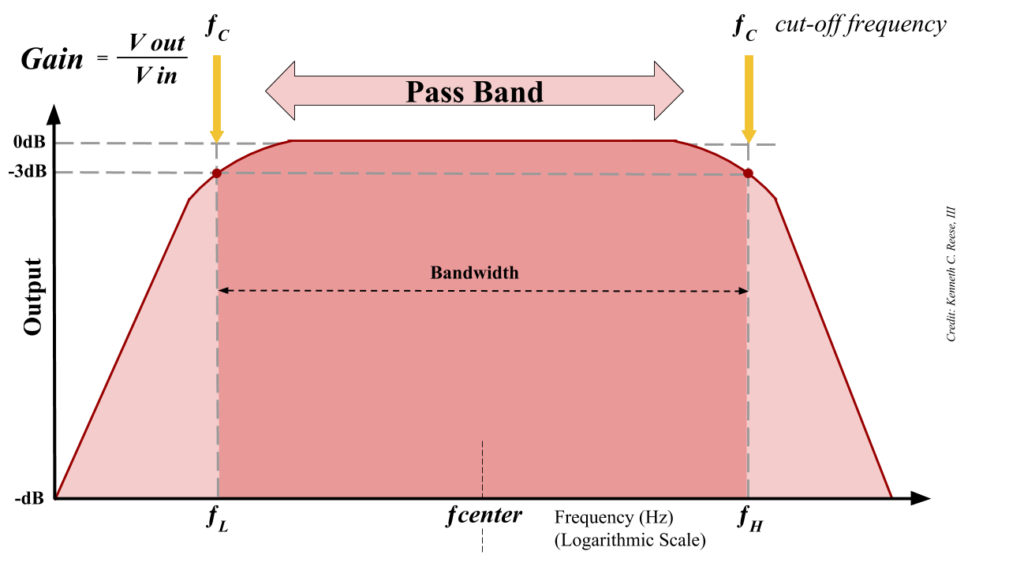
\includegraphics[width=0.7\textwidth]{3.Conceptos_Previos/bandpass-filter-fig-1-1024x577-2751970399.png}
    \caption{Filtrado de las frecuencias.\\ Fuente:\cite{Reeve2024BandPass}.}
    \label{fig:bandpass}
\end{figure}

La anchura de banda debe ser lo suficientemente estrecha para aislar las líneas de absorción de interés, pero lo suficientemente ancha para mantener una SNR adecuada. Los filtros deben tener alta transmitancia en la banda de interés para maximizar la señal y baja transmitancia fuera de banda para evitar contaminación espectral. Así mismo deben ser capaces de bloquear al máximo el resto de las bandas fuera de nuestro interés para reducir el ruido.

\subsubsection*{Tipos de Filtros y Configuración}


\begin{itemize}
    \item \textbf{Rueda de filtros}: Un solo detector y una rueda que posiciona secuencialmente diferentes filtros delante del detector. Es una solución asequible pero introduce partes móviles y puede limitar la velocidad de adquisición.
    
    \item \textbf{Módulos de filtro independientes}: Cada detector tiene su propio filtro fijo. Permite mayor robustez y elimina partes móviles, pero puede aumentar el tamaño del plano focal y dificultar la corregistración espacial.
    
    \item \textbf{Filtros tipo \textit{microstrip}}: Filtros miniaturizados directamente sobre el detector o muy próximos a él. Permiten una disposición compacta y robusta, adecuada para configuraciones multiespectrales con alta corregistración.
\end{itemize}





\section{Parámetros Orbitales}


\begin{figure}[H]
    \centering
    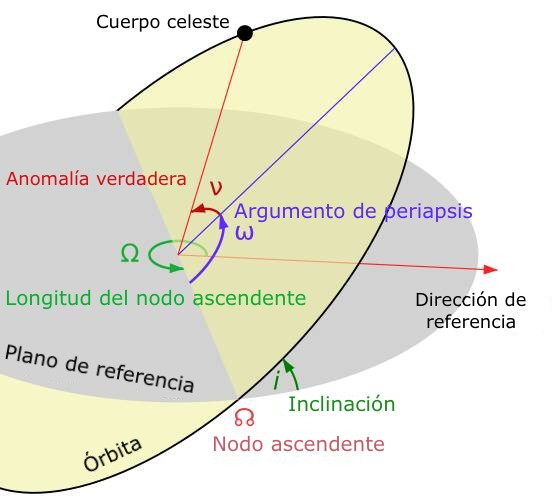
\includegraphics[width=0.5\linewidth]{3.Conceptos_Previos/Elementos_orbitales.jpg}
    \caption{Representación gráfica de los elementos orbitales. \\ Fuente: \cite{WikiElementosOrbitales}.
}
\end{figure}

A continuación se definen los principales parámetros que definen la órbita del cuerpo de interés, así como las perturbaciones asociadas de mayor peso en la mecánica orbital para el presente problema \cite{curtis2020orbital}.

\subsubsection*{Semieje mayor ($a$)}

El semieje mayor determina el tamaño básico de la órbita elíptica, representando la distancia desde el centro de la elipse hasta su extremo más alejado sobre el eje principal.

\subsubsection*{Excentricidad ($e$)}

La excentricidad define la forma de la órbita, como la desviación del cuerpo central respecto al centro geométrico de la elipse. Matemáticamente:

\begin{align}
e = \sqrt{1 - \frac{b^2}{a^2}}
\end{align}

donde \( b \) es el semieje menor. La excentricidad determina varios tipos de órbitas:

\begin{itemize}
    \item \( e = 0 \): Órbita perfectamente circular
    \item \( 0 < e < 1 \): Órbita elíptica (como la mostrada en las imágenes)
    \item \( e = 1 \): Trayectoria parabólica
    \item \( e > 1 \): Trayectoria hiperbólica
\end{itemize}

\noindent Estos parámetros no tendrán mucha relevancia en este trabajo como veremos más adelante, ya que por simplicidad escogeremos una orbita circular$(e\approx0)$. El semieje mayor se podrá resumir en la altura orbital,
definida como $h= a- R_T$, siendo $R_T$ el radio de la Tierra.

\subsection{Inclinación ($i$)}

La inclinación representa el ángulo entre el plano orbital y el plano de referencia (generalmente el ecuador terrestre). En la primera imagen se muestra como el ángulo formado entre estos dos planos. Para órbitas terrestres, se clasifica de la siguiente manera:

\begin{itemize}
  \item $i = 0^\circ$: Órbita ecuatorial
  \item $0^\circ < i < 90^\circ$: Órbita prógrada
  \item $i = 90^\circ$: Órbita polar
  \item $90^\circ < i < 180^\circ$: Órbita retrógrada
\end{itemize}

Este parámetro es crucial para determinar qué regiones de la Tierra sobrevolará el satélite.

\subsection{Longitud del Nodo Ascendente ($\Omega$)}

La longitud del nodo ascendente define la orientación del plano orbital en el espacio tridimensional. Como se visualiza en la primera imagen, es el ángulo medido desde la dirección de referencia hasta el nodo ascendente (punto donde la órbita cruza el plano de referencia en dirección norte). Este elemento es particularmente importante para órbitas heliosíncronas, donde precesa aproximadamente $1^\circ$ diario para mantener una relación constante con el Sol.

\subsection{Hora de paso local (LTAN)}

La hora de paso local en el nodo ascendente (\textit{Local Time of Ascending Node}, o LTAN) es el instante del día, medido en tiempo solar local, en que el satélite cruza el meridiano de su nodo ascendente. Es fundamental para misiones de observación de la Tierra, ya que determina las condiciones de iluminación solar en cada pasada.

Se calcula relacionando la longitud ascendente $\Omega$ con la posición del Sol en longitud eclíptica $\lambda_\odot(t)$, según:
\[
T_{\mathrm{LST}} 
= \frac{\Omega - \lambda_\odot(t)}{15^\circ}\quad[\mathrm{horas}],
\]
donde:
\begin{itemize}
  \item $\Omega$ es la longitud del nodo ascendente (°),
  \item $\lambda_\odot(t)$ es la longitud eclíptica del Sol en el instante $t$ (°),
  \item el factor $15^\circ/$h convierte grados en horas solares locales.
\end{itemize}

En la práctica se suele referir el LTAN a valores redondeados (por ejemplo, 10:30 h o 13:30 h) para garantizar escenas con sombras y contraste adecuados. En órbitas heliosíncronas, la precesión de $\Omega$ ($\approx$ 1º/día) se ajusta de modo que el LTAN permanezca prácticamente constante durante toda la misión.


\subsection{Argumento del Perigeo ($\omega$)}

El argumento del perigeo describe la orientación de la elipse dentro del plano orbital. En las figuras se muestra como el ángulo entre el nodo ascendente y el punto de máximo acercamiento al cuerpo central (perigeo). Este parámetro determina dónde se producirán las distancias mínima y máxima de la órbita. Para satélites científicos en órbitas excéntricas, este valor se elige cuidadosamente para sobrevolar determinadas regiones a la altura mínima. 

Debido a que en este estudio solo se aplicaran orbitas circulares ($e\approx0$), este parámetro carece de relevancia, pues no habrá un perigeo claramente definido.

\subsection{Anomalía Verdadera ($\nu$)}

La anomalía verdadera es el único elemento que varía con el tiempo para una órbita no perturbada. Representa la posición instantánea del cuerpo orbitante, medida como el ángulo desde el perigeo hasta la posición actual del satélite, en la dirección del movimiento.


\section{Perturbaciones de la órbita}

\subsection{Achatamiento Terrestre}

La Tierra no es perfectamente esférica; presenta un abultamiento en el ecuador debido a su rotación. Este achatamiento genera un campo gravitacional asimétrico que introduce una perturbación en las órbitas de los satélites. Este efecto provoca dos movimientos importantes en los elementos orbitales:

\begin{enumerate}
    \item \textbf{Regresión del nodo ascendente} (\( \Omega \)): El nodo ascendente, el punto donde la órbita cruza el ecuador de sur a norte, experimenta un movimiento de precesión regresiva.
    \item \textbf{Precesión del argumento del perigeo} (\( \omega \)): El argumento del perigeo también se ve afectado, lo cual es relevante para órbitas con cierta excentricidad.
\end{enumerate}

Estas perturbaciones dependen de la altitud, la inclinación y otros parámetros orbitales. En el próximo apartado (\ref{sec:SSO}) se detalla como acoplar dichas variables para definir órbitas heliosíncronas.



\subsection{Decaimiento Orbital}


\begin{figure}[H]
    \centering
    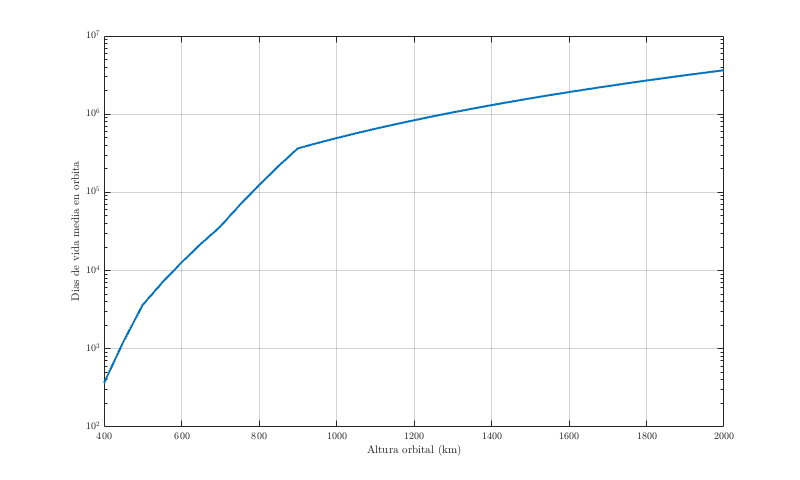
\includegraphics[width=0.9\textwidth]{3.Conceptos_Previos/Diasvidamediaorbitavsaltitud.png} 
    \caption{Días de vida media en órbita vs Altura orbital (km).\\ Fuente: Elaboración propia basada en \cite{spaceacademy_orblife}.}
    \label{fig:vida_media_orbita}
\end{figure}

Los satélites en órbita baja terrestre (LEO), típicamente por debajo de los 1000 km de altitud, están expuestos a una atmósfera tenue pero no nula. A esas alturas, aún existen partículas atmosféricas que ejercen una fuerza de arrastre sobre el satélite a medida que este se desplaza a velocidades orbitales. Este arrastre provoca una pérdida continua de energía orbital,  que hace que el satélite descienda gradualmente a órbitas más bajas. Este fenómeno se conoce como \textbf{decaimiento orbital}.

Con el tiempo, un satélite que no cuenta con sistemas de propulsión para mantener su altitud experimentará una disminución continua de su altura orbital, reingresando eventualmente en la atmósfera densa, donde se desintegrará por el calor generado por la fricción. Este mecanismo actúa también como forma pasiva de mitigación de desechos espaciales, lo cual será interesante tener en consideración una vez llegue el fin de vida del satélite.

\subsection{Radiación Solar}

La radiación solar está compuesta por partículas (fotones) que viajan a la velocidad de la luz. Estos fotones, aunque no tienen masa, sí tienen energía y cantidad de movimiento. 

Cuando los fotones de la radiación solar golpean un objeto, como un satélite, se produce una transferencia de momento del fotón al objeto. Esta pequeña fuerza es la presión de radiación.

Aunque la presión es pequeña, para satélites con grandes superficies expuestas (como los que tienen paneles solares grandes o velas solares), puede producirse una desviación progresiva de la órbita. Puede cambiar el argumento del perigeo, haciendo que la órbita se desplace gradualmente.


\subsection{Problema del tercer cuerpo}

El problema del tercer cuerpo se refiere a la dinámica gravitacional que surge cuando tres objetos celestes (en nuestro caso, el sistema Tierra-Luna- satélite, o Tierra-Sol- satélite) interactúan entre sí mediante la fuerza de gravedad. A diferencia del problema de dos cuerpos, que tiene una solución matemática exacta y predecible, la adición de un tercer cuerpo introduce un nivel de complejidad significativo.

Cuando solo dos cuerpos interactúan gravitacionalmente, sus movimientos forman órbitas estables y predecibles. Sin embargo, cuando se introduce un tercer cuerpo, este genera perturbaciones en las órbitas que serían estables en el caso de dos cuerpos.

El tratamiento analítico de este problema es extraordinariamente difícil porque la perturbación depende explícitamente del tiempo. Las ecuaciones diferenciales que describen este sistema no tienen una solución cerrada o analítica exacta, lo que ha lleva al desarrollo de métodos numéricos para aproximar las soluciones.

El sistema de tres cuerpos es intrínsecamente caótico, lo que significa que es extremadamente sensible a las condiciones iniciales. Pequeñas variaciones en la posición o velocidad inicial de cualquiera de los cuerpos pueden resultar en trayectorias completamente diferentes a largo plazo. Esto imposibilita predicciones precisas sin conocer con exactitud absoluta las condiciones iniciales.\\

\subsection{Órbitas de especial interés}

\subsubsection{Órbitas heliosíncronas}\label{sec:SSO}

Las órbitas heliosíncronas son aquellas en las que el plano orbital mantiene una orientación constante respecto al Sol. Esto permite que el satélite pase sobre cualquier punto de la Tierra a la misma hora solar local, asegurando condiciones de iluminación consistentes para aplicaciones como monitoreo ambiental y teledetección.

El efecto del achatamiento terrestre es clave para lograr esta sincronización. La regresión nodal inducida por el achatamiento puede ajustarse seleccionando adecuadamente la altitud y la inclinación orbital. Para una órbita heliosíncrona, la velocidad angular de precesión del nodo ascendente debe coincidir con la velocidad angular aparente del Sol respecto a la Tierra (\( \approx 0.9856^\circ/\text{día} \)). Con esto se obtiene la ecuación que dará la inclinación de la órbita en función de la altura:

\begin{align}
\cos i = -\frac{2 r^{7/2} \, \omega_{\text{sol}}}{3 J_2 R_T^2 \sqrt{\mu}}
\end{align}

\noindent donde:

\begin{itemize}
    \item \( i \) es la inclinación orbital,
    \item \( r \) es el radio orbital (radio de la Tierra + altitud del satélite),
    \item \( \omega_{\text{sol}} \approx 1.991 \times 10^{-7} \ \text{rad/s} \) es la velocidad angular aparente del Sol respecto a la Tierra,
    \item \( J_2 \approx 1.08263 \times 10^{-3} \) es el coeficiente zonal que representa el achatamiento terrestre,
    \item \( R_T \approx 6378.1 \ \text{km} \) es el radio medio de la Tierra,
    \item \( \mu \approx 3.986 \times 10^{14} \ \text{m}^3/\text{s}^2 \) es la constante gravitacional estándar de la Tierra.
\end{itemize}

\subsubsection{Órbitas de Traza Repetida}


Una órbita de traza repetida (RGT o \textit{Repeating Ground Track}) es aquella en la que el satélite repite su proyección sobre la superficie terrestre después de un número entero de días \( D \) y un número entero de órbitas \( N \). Estas órbitas son especialmente útiles para misiones de observación terrestre, ya que permiten adquirir imágenes de una misma zona bajo condiciones geométricas similares a intervalos regulares.

El criterio para una órbita RGT se establece a partir de la sincronización entre el período orbital \( T_{\mathrm{orb}} \) del satélite y la rotación de la Tierra. La condición matemática que debe cumplirse es:

\begin{equation}
N \cdot T_{\mathrm{orb}} = D \cdot T_{\mathrm{sidereal}}
\end{equation}

donde:
\begin{itemize}
    \item \( N \in \mathbb{N} \): número de órbitas completas en \( D \) días,
    \item \( T_{\mathrm{orb}} \): período orbital del satélite,
    \item \( D \in \mathbb{N} \): número de días (normalmente días solares o sidéreos),
    \item \( T_{\mathrm{sidereal}} = 86164 \, \si{s} \): duración del día sidéreo terrestre.
\end{itemize}


Utilizando la tercera ley de Kepler, se relacionan la altitud orbital y periodo orbital

\begin{equation}
T_{\mathrm{orb}} = 2\pi \sqrt{\frac{(R_T + H)^3}{\mu}}
\end{equation}

De este modo, se obtiene la altitud \( H \) que satisface la condición de repetición. Esta clase de órbitas permite optimizar la planificación de coberturas periódicas.



\subsection{Consideración de las perturbaciones orbitales}


Para el presente trabajo no se considera la radiación solar ni el problema del tercer cuerpo, a fin de simplificar los cálculos necesarios. Esto no es descabellado, ya que, como se verá mas adelante, se evaluará una órbita baja (\textit{Low Earth Orbit}, o LEO ) en la cual la influencia de la gravedad terrestre será en ordenes de magnitud mayores a cualquier otro cuerpo celeste cercano (como la Luna o el Sol). También significa que el telescopio no será excesivamente grande, ni, por ende, el resto de subsistemas, por lo que la fuerza generada por la presión de radiación será de un valor ínfimo. No obstante, esta proximidad a la Tierra hará que la fricción con la atmósfera si sea una perturbación a considerar en el diseño de la misión. Así mismo, el achatamiento terrestre también será fundamental a la hora de considerar órbitas heliosíncronas.